\documentclass[num-refs]{wiley-article}

\usepackage{graphicx}
\usepackage[space]{grffile}
\usepackage{latexsym}
\usepackage{textcomp}
\usepackage{longtable}
\usepackage{tabulary}
\usepackage{booktabs,array,multirow}
\usepackage{amsfonts,amsmath,amssymb}
\usepackage{natbib}
\usepackage{url}
\usepackage{hyperref}
\hypersetup{colorlinks=false,pdfborder={0 0 0}}
% You can conditionalize code for latexml or normal latex using this.
\newif\iflatexml\latexmlfalse
\providecommand{\tightlist}{\setlength{\itemsep}{0pt}\setlength{\parskip}{0pt}}%

\AtBeginDocument{\DeclareGraphicsExtensions{.pdf,.PDF,.eps,.EPS,.png,.PNG,.tif,.TIF,.jpg,.JPG,.jpeg,.JPEG}}

\usepackage[utf8]{inputenc}
\usepackage[english]{babel}

% Add any additional LaTeX packages and macros here
\usepackage{siunitx}
\usepackage{placeins}
\usepackage{xcolor}
\usepackage{float}

% Define command for Fabio's comments in red
\newcommand{\fabio}[1]{\textcolor{red}{[#1]}}

%---

\iflatexml
% Add any LateXML specific commands here

%---

\else
% The commands below will only change the exported PDF. Edit or remove as needed

\paperfield{Clinical Neurology}
\abbrevs{GLMM, generalized linear mixed model; KSS, Kahneman-Sibony-Sunstein; LTM, latent trait model; MCMC, Markov chain Monte Carlo.}
\corraddress{M. Brandon Westover MD PhD, Department of Neurology, Massachusetts General Hospital, Harvard Medical School, Boston, MA, USA}
\corremail{mwestover@mgh.harvard.edu}
\fundinginfo{National Institutes of Health, Grant/Award Numbers: R01AG073410, R01HL161253, R01NS126282, R01AG073598, R01NS131347, R01NS130119}
\fi

%---

\papertype{Original Article}

\title{How to Analyze Noise in Medical Decision Making}

\author[1]{Fábio A. Nascimento}
\affil[1]{Washington University School of Medicine in St. Louis}

\author[1]{Xuming He}
\affil[1]{Washington University School of Medicine in St. Louis}

\author[2]{Jin Jing}
\affil[2]{Harvard Medical School}

\author[2]{M. Brandon Westover}
\affil[2]{Harvard Medical School}

\runningauthor{M. Brandon Westover}

\begin{document}

\raggedbottom  % Prevent LaTeX from stretching vertical space to fill pages

\maketitle
\selectlanguage{english}

\begin{abstract}
\textbf{Background:} When multiple clinicians evaluate the same cases, disagreement arises from various forms of noise: differences between-clinicians in systematic biases (level noise), idiosyncratic case-by-rater interactions (pattern noise), and within-clinician inconsistency (occasion noise). The observed variation in responses across cases reflects both the underlying signal (genuine differences between cases) and these noise sources. Traditional reliability metrics collapse all disagreement into a single number, preventing identification of specific noise sources.

\textbf{Methods:} We present a unified statistical framework for decomposing variation in binary medical decisions. We show that the latent trait model (LTM) and the Kahneman-Sibony-Sunstein (KSS) noise decomposition are special cases of a generalized linear mixed model. We use Bayesian estimation via Markov chain Monte Carlo to obtain posterior distributions for all variance components and their relative contributions. We demonstrate the approach using data from epilepsy diagnosis and EEG interictal epileptiform discharge (IED) classification.

\textbf{Results:} In an epilepsy diagnosis study with 20 board-certified epileptologists reviewing 50 cases on two occasions, system noise (level + pattern + occasion) accounted for 31-34\% of total variation. Based on clinical history alone, level noise (systematic bias) was the dominant component (23\%). After incorporating EEG and neuroimaging results, pattern noise (idiosyncratic case interpretations) became dominant (24\%), while level noise decreased to 5\%. Occasion noise remained minimal (1\%) despite 16\% of cases showing diagnostic reversals between occasions. Diagnostic accuracy was 71\% overall, but only 56\% for difficult cases.

\textbf{Conclusions:} The noise decomposition framework provides actionable insights into sources of diagnostic disagreement. By separating level, pattern, and occasion noise, researchers can design targeted interventions (e.g., threshold calibration for level noise, case-based training for pattern noise, decision aids for occasion noise). We provide practical guidance on sample size requirements, model implementation, and interpretation for applied medical researchers.

\textbf{Keywords} --- inter-rater reliability, noise decomposition, signal detection theory, generalized linear mixed models, Bayesian hierarchical models, diagnostic disagreement%
\end{abstract}

% Main content sections
\section*{Introduction}
\label{707961}

Medical decision-making is a complex cognitive process in which clinicians interpret clinical information and arrive at diagnostic or treatment decisions. Disagreement among professionals is common, even when they evaluate the same data. Understanding the sources of this disagreement is essential for improving diagnostic reliability and accuracy, designing effective training interventions, and determining appropriate sample sizes in clinical research.

Inter- and intra-rater disagreement reflects both (i) variation in the underlying signal (i.e., genuine differences in case difficulty) and (ii) noise (i.e., unwanted variability in judgment). Traditional reliability metrics such as Cohen’s kappa or intraclass correlation coefficients quantify \textit{how much} experts disagree, but they provide little insight into \textit{why}. For example, a kappa of 0.65 indicates “moderate agreement,” yet it does not indicate whether disagreement arises from differing thresholds, idiosyncratic feature weighting, instability within raters over time, or random inconsistency. Without identifying the sources of disagreement, it is difficult to design targeted interventions to improve reliability and accuracy.

Recent work in decision science \cite{Kahneman2021} distinguishes multiple types of noise: \textit{level noise} (systematic differences in how lenient or stringent raters are), \textit{pattern noise} (idiosyncratic differences in how raters weigh features of individual cases), and \textit{occasion noise} (inconsistency within the same rater across repeated assessments of identical information). Each noise type suggests different remedies: level noise motivates threshold calibration, pattern noise motivates case-based training, and occasion noise motivates environmental controls or decision support tools.

Consider two clinicians who disagree on whether a patient has epilepsy. Is the disagreement because one clinician is generally more conservative (level noise), because they weight clinical evidence differently (pattern noise), or because one clinician is inconsistent across repeated assessments (occasion noise)? Standard agreement metrics cannot distinguish among these possibilities. This paper provides a “diagnostic tool for diagnostic systems”: a framework that decomposes disagreement into interpretable, actionable components.

We present a unified statistical framework for quantifying sources of variation in binary medical decisions such as “Does this patient have epilepsy?” or “Is this waveform epileptiform?” We show that the latent trait model (LTM) and the Kahneman--Sibony--Sunstein (KSS) noise decomposition framework can be understood as special cases of a single generalized linear mixed model (GLMM). We demonstrate the framework using data from an experiment in which 20 expert neurologists evaluated 50 cases for epilepsy diagnosis \cite{nascimentonoise}. We provide practical guidance for applied researchers on model implementation, interpretation, and study design. A key result is that discrimination ability (as measured by area under the ROC curve) depends only on pattern and occasion noise, whereas threshold choice (the operating point on the ROC curve) is governed by level noise.

\subsection*{Overview: Inputs, Outputs, and Use Cases}

To orient applied readers, we summarize what the method requires, what it produces, and when it is useful.

\begin{table}[h!]
\centering
\small
\begin{tabular}{p{0.25\textwidth}p{0.65\textwidth}}
\toprule
\textbf{Component} & \textbf{Description} \\
\midrule
\multicolumn{2}{l}{\textbf{INPUTS}} \\
Binary ratings & Response array $Y_{ijt}$: ratings from $M$ raters on $N$ cases, optionally repeated over $T$ occasions \\
Sample sizes & Typical: $N \geq 30$ cases, $M \geq 10$ raters; $T \geq 2$ occasions if estimating occasion noise \\
Gold standard (optional) & Reference labels for evaluating accuracy (sensitivity/specificity); not required for noise decomposition \\
\midrule
\multicolumn{2}{l}{\textbf{PRIMARY OUTPUTS}} \\
Variance components & Standard deviations $\sigma_c, \sigma_\ell, \sigma_p, \sigma_o$ quantifying signal, level noise, pattern noise, and occasion noise \\
Percent contributions & Proportion of total variation explained by each component \\
Uncertainty & Credible intervals (Bayesian) or confidence intervals (frequentist) for all estimates \\
\midrule
\multicolumn{2}{l}{\textbf{SECONDARY OUTPUTS}} \\
Rater-level summaries & Individual estimates of level noise, pattern noise, occasion noise for each rater \\
Case-level summaries & Predicted consensus probability for each case \\
Model validation & Posterior predictive checks, goodness-of-fit diagnostics \\
\midrule
\multicolumn{2}{l}{\textbf{USE CASES}} \\
1. Quantify disagreement & Separate signal from noise; identify specific noise sources \\
2. Compare groups & Test whether/how experts vs.\ non-experts differ in level, pattern, or occasion noise \\
3. Design studies & Determine required sample sizes (cases, raters, repeats) \\
4. Evaluate training & Measure changes in noise components before/after training interventions \\
5. Quality assurance & Identify raters with excessive noise or miscalibration \\
\bottomrule
\end{tabular}
\caption{Summary of inputs, outputs, and use cases for the noise decomposition framework.}
\label{tab:overview}
\end{table}

\subsection*{Why Decomposition Matters: An Illustrative Example}

Figure~\ref{fig:killer} illustrates why decomposing noise into its components is clinically valuable. We simulated two raters evaluating the same cases on three occasions, assuming equal numbers of positive and negative cases but varying case difficulty. The variation in the underlying signal (degree of evidence pointing to the correct diagnosis) is represented by $\sigma_c$. Both raters see identical information, but their judgments are affected by different amounts and types of noise:

\beg


% \section*{Introduction}

% {\label{707961}}

% Medical decision-making refers to the complex cognitive process whereby medical professionals interpret clinical information and arrive at diagnostic or treatment decisions. Disagreement among professionals in making medical decisions is not uncommon. Understanding the sources of this disagreement is critical for improving diagnostic reliability and accuracy, designing clinical training programs, and determining appropriate sample sizes in clinical research.

% Inter- and intra-rater disagreement arises both from noise (i.e., unwanted variability) and the underlying signal (i.e., variability derived from genuine differences in case difficulty). While traditional reliability metrics such as Cohen's kappa or intraclass correlation coefficients tell us \textit{how much} experts disagree, they fail to inform us why. For instance, a kappa of 0.65 indicates ``moderate agreement'', but provides no insight into whether disagreement stems from varying case difficulty, differing personal thresholds, idiosyncratic interpretations of evidence, or random inconsistency. Without understanding the precise sources of disagreement, we cannot design targeted interventions to improve accuracy and reliability.

% Recent work in decision science \cite{Kahneman2021} has identified distinct types of noise: \textit{level noise} (systematic differences in how lenient or stringent raters are), \textit{pattern noise} (idiosyncratic differences in how raters weigh features of individual cases), and \textit{occasion noise} (inconsistency within the same rater across repeated assessments of the same data). Crucially, each noise type suggests different remedies: level noise calls for threshold calibration, pattern noise for case-based training, and occasion noise for environmental control and decision support tools.

% Consider two clinicians who disagree on whether a patient has epilepsy. Is the disagreement because one expert is generally more conservative in diagnosing epilepsy (level noise), or because they give different weights to different aspects of the case (pattern noise), or because one expert is having an "off day" (occasion noise)? Traditional reliability metrics cannot answer this question. This paper provides a "diagnostic tool for diagnostic systems"--- a framework to decompose disagreement into quantifiable, actionable components.

% We present a unified statistical framework for quantifying the sources of variation in binary medical decisions such as, "Does this patient have epilepsy?" or "Is this waveform epileptiform?". We show how the latent trait model (LTM) and the Kahneman-Sibony-Sunstein (KSS) noise decomposition framework can be understood as special cases of a single generalized linear mixed model (GLMM). We demonstrate the framework using data from an experiment where 20 expert neurologists evaluated 50 cases for epilepsy diagnosis \cite{nascimentonoise}. We provide practical guidance for applied researchers on how to implement these models, interpret the results, and design studies to estimate noise components reliably. We show that discrimination ability (reflected in the area under the ROC curve) depends only on pattern noise and occasion noise, while threshold choice (the operating point on the ROC curve) is determined by level noise.

% \subsection*{Overview: Inputs, Outputs, and Use Cases}

% To orient applied readers, we first summarize what this method requires, what it produces, and when it is useful.

% \begin{table}[h!]
% \centering
% \small
% \begin{tabular}{p{0.25\textwidth}p{0.65\textwidth}}
% \toprule
% \textbf{Component} & \textbf{Description} \\
% \midrule
% \multicolumn{2}{l}{\textbf{INPUTS}} \\
% Binary ratings & Response array $Y_{ijt}$: ratings from $M$ raters on $N$ cases, optionally repeated over $T$ occasions \\
% Sample sizes & Typical: $N \geq 30$ cases, $M \geq 10$ raters; $T \geq 2$ occasions if estimating occasion noise \\
% Gold standard (optional) & Reference labels for evaluating accuracy (sensitivity/specificity); not required for noise decomposition \\
% \midrule
% \multicolumn{2}{l}{\textbf{PRIMARY OUTPUTS}} \\
% Variance components & Standard deviations $\sigma_c, \sigma_\ell, \sigma_p, \sigma_o$ quantifying signal, level noise, pattern noise, and occasion noise \\
% Percent contributions & Proportion of total variation explained by each component \\
% Uncertainty & Credible intervals (Bayesian) or confidence intervals (frequentist) for all estimates \\
% \midrule
% \multicolumn{2}{l}{\textbf{SECONDARY OUTPUTS}} \\
% Rater-level summaries & Individual estimates of level noise, pattern noise, occasion noise for each rater \\
% Case-level summaries & Predicted consensus probability for each case \\
% Model validation & Posterior predictive checks, goodness-of-fit diagnostics \\
% \midrule
% \multicolumn{2}{l}{\textbf{USE CASES}} \\
% 1. Quantify disagreement & Separate signal from noise; identify specific noise sources \\
% 2. Compare groups & Test whether/how experts vs. non-experts differ in level, pattern, or occasion noise \\
% 3. Design studies & Determine required sample sizes (cases, raters, repeats) \\
% 4. Evaluate training & Measure changes in noise components before/after training interventions \\
% 5. Quality assurance & Identify raters with excessive noise or miscalibration \\
% \bottomrule
% \end{tabular}
% \caption{Summary of inputs, outputs, and use cases for the noise decomposition framework.}
% \label{tab:overview}
% \end{table}

% \subsection*{Why Decomposition Matters: An Illustrative Example}

% Figure~\ref{fig:killer} illustrates why decomposing noise into its components is clinically valuable. We simulated two raters evaluating the same cases, on three occasions. We assume an equal number of positive and negative cases, but that case difficulty varies, and the variation in the underlying signal (degree of evidence pointing to the correct diagnosis) is represented by $\sigma_c$. The two raters see the same information, but their judgments are clouded by different anmounts and types of noise:

% \begin{itemize}
%     \item \textbf{Rater A ("Stringent but consistent"):} Low pattern noise ($\sigma_p = 0.66$) and occasion noise ($\sigma_o = 0.44$) result in \textit{superior} discrimination (AUC = 0.78)---this rater has substantially better ability to distinguish positive from negative cases compared to rater B. However,  rater A has a systematically conservative threshold ($\ell = 2.0$), yielding low sensitivity (29\%) and high specificity (95\%, FPR = 5\%), with overall accuracy of 62\%. If this rater adjusted their threshold to the optimal value, they could achieve 71\% accuracy; they are wasting 9 percentage points of potential accuracy due to systematic underdiagnosis. This demonstrates that threshold optimization alone can improve accuracy without changing discrimination ability.

%     \item \textbf{Rater B ("Lenient but inconsistent"):} Lower skill, reflected in higher pattern noise ($\sigma_p = 0.97$) and occasion noise ($\sigma_o = 0.65$) result in \textit{inferior} discrimination (AUC = 0.70)---rater B's ability to distinguish positive from negative cases is worse than Rater A's. However, this rater has a well-calibrated threshold ($\ell = 0.2$), producing balanced sensitivity (64\%) and specificity (64\%, false positive rate = 36\%), yielding accuracy of 64\%, better than Rater A. Rater B is already operating at their optimal threshold and cannot improve accuracy without improving in skill, which means reducing discrimination noise (by reducing pattern and occasion noise). This shows that inferior discrimination with an optimal threshold can yield higher accuracy than superior discrimination with a miscalibrated threshold.
% \end{itemize}

% The heatmaps of responses (cases × occasions) in Figure 1 reveal the distinct noise patterns. Rater A shows systematic bias (a tendancy to undercall the positive class), while Rater B shows scattered disagreements. The ROC curves demonstrate that Rater A has the better ROC curve (higher AUC due to low pattern noise and occasion noise) but operates at a suboptimal point (white circle) due to conservative bias. Rater B has the worse ROC curve (lower AUC due to high pattern noise and occasion noise) but operates at a more well-calibrated point (black circle) due to unbiased threshold. Operating points show each rater's sensitivity-specificity trade-off.

% The stacked bars show signal and discrimination noise (pattern + occasion) as percentages of total response variance for each rater. Both raters see the same signal (same cases), but the percentages differ because they are relative to each rater's total variance. Rater A has lower total variance due to low discrimination noise, making signal represent a larger proportion. Rater B has higher total variance due to high discrimination noise. The variance decomposition reveals discrimination ability: Rater A has better discrimination (lower proportion of total response variation attributable to pattern and occasion noise) but an overly conservative threshold, while Rater B has poor discrimination (higher proportion of response variation explained by pattern and occasion noise) but good threshold calibration.

% \textbf{Clinical implications:}
% \begin{itemize}
%     \item For Rater A: Threshold recalibration (e.g., anchoring vignettes, feedback on diagnostic under-calling tendencies) is \textit{high priority}. The superior discrimination ability (AUC = 0.78) is being wasted due to a systematically very conservative threshold. Correcting the bias would improve accuracy from 62\% to 71\% (recovering 9 percentage points) without any change in discrimination (pattern noise and occasion noise). This is a \textit{low-cost, high-impact} intervention---no additional training required, just threshold adjustment. The large "wasted" potential (9 points) makes this especially urgent.
%     \item For Rater B: Case-based training (to reduce pattern noise) and decision aids (to reduce occasion noise) would improve discrimination, but are higher-cost interventions. Rater B is already operating at their optimal threshold (64\% accuracy), so they cannot improve further without reducing discrimination noise (pattern noise and occasion noise). Improving discrimination from AUC 0.70 to 0.78 would increase accuracy from 64\% to 71\%; however, this requires intensive training, unlike Rater A's "simple" threshold fix.
%     \item Traditional metrics focusing only on agreement or consistency would suggest Rater A is superior (less variable, higher AUC), missing that Rater A's superior discrimination is being undermined by poor threshold calibration while Rater B's inferior discrimination is being maximally utilized by optimal threshold choice. 
%     \item The key insight: Superior discrimination does not guarantee higher accuracy if threshold choice is suboptimal; conversely, inferior discrimination can yield higher accuracy if threshold choice is optimal. Noise decomposition reveals \textit{where} to intervene and \textit{how much} potential is being "wasted"---not just that intervention is needed.
% \end{itemize}

% In the example above, we have been comparing two individual clinicians, attributing their tendency to under- or over-diagnose cases as a fixed threshold, $\ell$, and we have noted that this threshold can vary between clinicians. When clinicians are viewed as a group, this unwanted threshold variation represents yet another form of noise, called \textit{level noise}. Thus, we have identified four sources of variation in the way clinicians may reach diagnoses: signal, and three sources of noise---level noise, pattern noise, and occasion noise. We now turn to how these can be measured and quantified.

% \begin{figure}[h!]
% \begin{center}
% 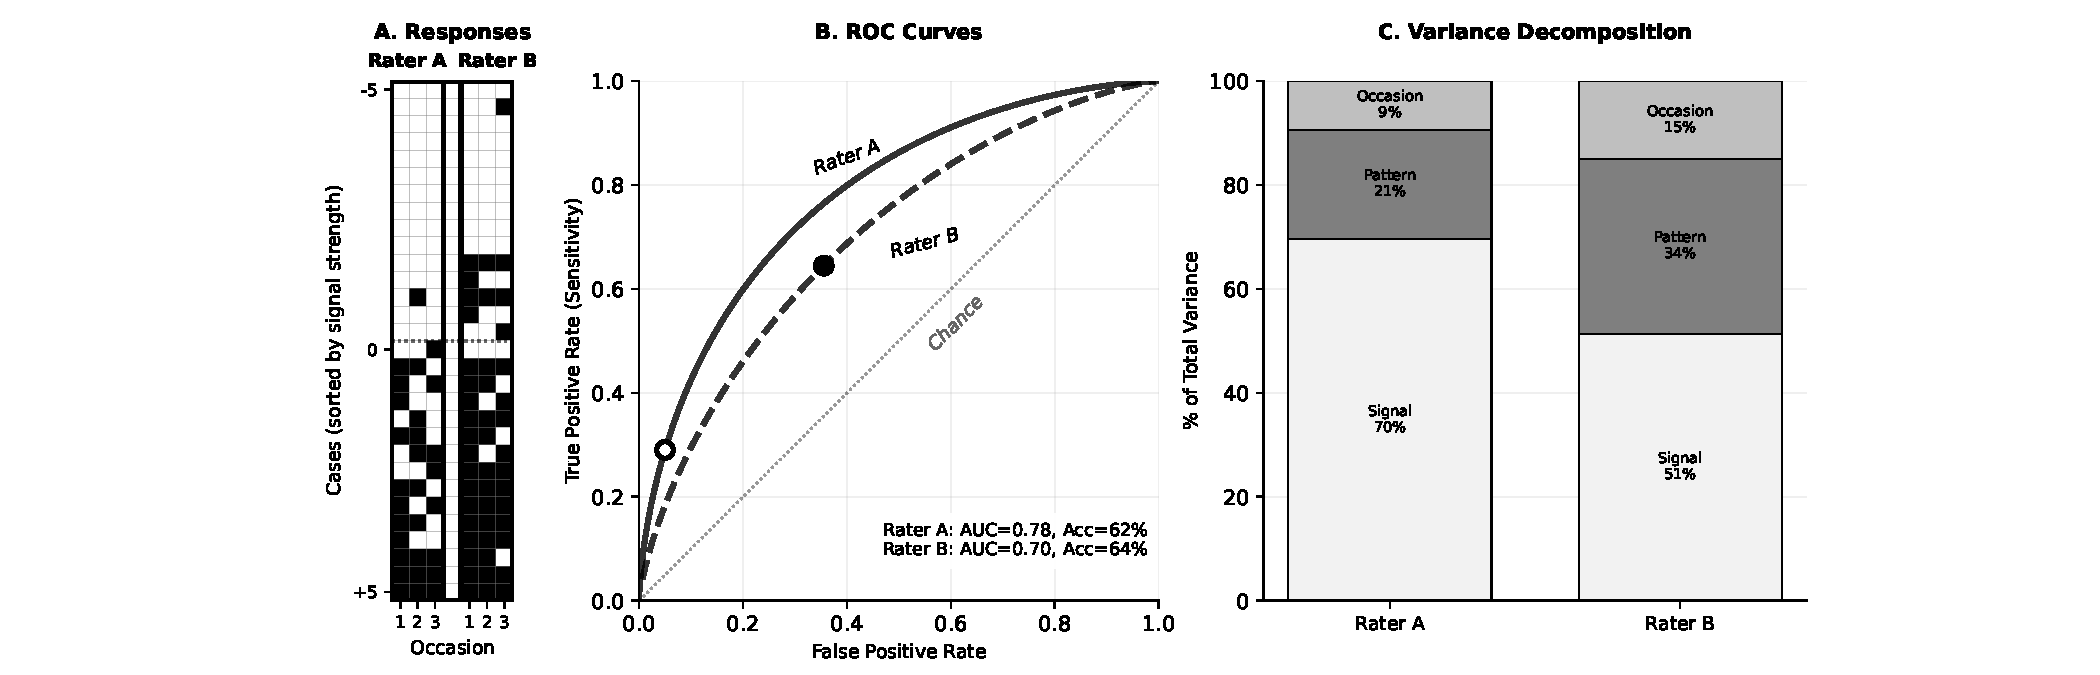
\includegraphics[width=1.0\textwidth]{killer_figure.pdf}
% \caption{\textbf{Superior discrimination with miscalibrated threshold yields lower accuracy than inferior discrimination with optimal threshold.} Two simulated raters evaluating the same cases (signal $\sigma_c = 1.2$ for both, prevalence = 50\%) with different noise profiles demonstrate why noise decomposition matters. \textbf{Panel A (Left):} Heatmaps of responses (30 cases × 3 occasions; white=negative, black=positive; cases sorted by difficulty; dotted line = true positive/negative boundary). Rater A (top) shows a clear tendency to under-call (systematic conservative bias), while Rater B (bottom) shows scattered disagreements reflecting inconsistency. \textbf{Panel B (Middle):} ROC curves from binormal model with discrimination ability (AUC) and actual accuracy (Acc) labeled on each curve. Rater A (solid line, AUC = 0.78) has substantially superior discrimination compared to Rater B (dashed line, AUC = 0.70). ROC curves reflect only pattern noise ($\sigma_p$) and occasion noise ($\sigma_o$)---\textit{not} threshold position ($\ell$). Operating points (circles) show where each rater operates on their respective curves. Rater A: low pattern noise ($\sigma_p = 0.66$) and occasion noise ($\sigma_o = 0.44$) yield superior discrimination (AUC = 0.78), but a systematically conservative threshold ($\ell = 2.0$) places them at a suboptimal operating point (white circle: sensitivity = 29\%, specificity = 95\%, FPR = 5\%), yielding only 62\% accuracy. With optimal threshold, this rater could achieve 71\% accuracy---\textit{wasting 9 percentage points due to threshold miscalibration}. Rater B: higher pattern noise ($\sigma_p = 0.97$) and occasion noise ($\sigma_o = 0.65$) yield inferior discrimination (AUC = 0.70), but a well-calibrated threshold ($\ell = 0.2$) produces a near-optimal operating point (black circle: sensitivity = 64\%, specificity = 64\%, FPR = 36\%), yielding 64\% accuracy---\textit{higher than Rater A despite worse discrimination}. Note that Rater A has higher AUC but lower accuracy than Rater B. \textbf{Panel C (Right):} Variance decomposition showing signal and discrimination noise as percentages of total response variance. Both raters see identical signal ($\sigma_c = 1.2$), but percentages differ because they are relative to each rater's total variance. Rater A has 54\% signal and 46\% discrimination noise (pattern + occasion); Rater B has 36\% signal and 64\% discrimination noise. The bars show only pattern and occasion noise (which together determine discrimination ability), not threshold position. The key insight: superior discrimination does not guarantee higher accuracy when threshold is miscalibrated. Appropriate interventions differ: threshold recalibration for Rater A (high priority, low-cost intervention recovering 9 percentage points) vs. case-based training to reduce pattern and occasion noise for Rater B (lower priority, high-cost intervention with modest gains).}
% \label{fig:killer}
% \end{center}
% \end{figure}


% \par\null


\section*{Two models of noise and skill}\label{2-models}

\subsection*{Notation}
Throughout this paper we use the following notation:
\begin{itemize}
    \item $i = 1,\ldots,N$ indexes cases (e.g., patient records, candidate waveforms)
    \item $j = 1,\ldots,M$ indexes raters
    \item $t = 1,\ldots,T$ indexes occasions (repeated ratings of the same case(s) by the same rater)
    \item $Y_{ijt}$ is the binary response (0 or 1) from rater $j$ on case $i$ at occasion $t$
\end{itemize}

We now explain the LTM and KSS models. Both models have this form: $Pr(Y_{ijt}=1) = f(z_{ijt})$, where $z_{ijt} = c_i + \ell_j + n_{ijt}$. Here, $Y_{ijt}=1$ represents a 'yes', 'positive', or 'correct' answer, depending on the context. The function $f$ can be either the logistic function $f(x) = 1/[1+\exp(-x)]$, or the cumulative Gaussian (probit) function $f(x) = (2\pi)^{-1/2}\int_{-\infty}^x \exp(-u^2/2)du$. The components of $z_{ijt}$ have somewhat different interpretations in the two models, which we explain below.

\subsection*{Latent Trait Model (LTM)}\label{section-LTM}
In the LTM,
\begin{eqnarray*}
  z_{ijt} &=& c_i + n_{ijt} \\
  Y_{ijt}&=&\begin{cases}
    1, & \text{if $z_{ijt}>\ell_j$}\\
    0, & \text{if $z_{ijt}\leq \ell_j$},
  \end{cases}
\end{eqnarray*}
where $c_i$ is the signal strength for case $i$ and $n_{ijt}$ is the noise. For an ideal observer, $z_{ijt} = c_i$, i.e., there is no noise ($n_{ijt}=0$). As indicated, decisions about the value of $Y_{ijt}$ are reached by comparing $z_{ijt}$ with a threshold value $\ell_j$ that is particular to rater $j$.

Note that a mathematically equivalent formulation is
\begin{eqnarray*}
  z_{ijt} &=& c_i - \ell_j + n_{ijt} \\
  Y_{ijt}&=&\begin{cases}
    1, & \text{if $z_{ijt}>0$}\\
    0, & \text{if $z_{ijt}\leq 0$},
  \end{cases}
\end{eqnarray*}
where we have absorbed $\ell_j$ into $z_{ijt}$. This form is consistent with the KSS model (see below) and with the logistic GLMM formulation where $\text{Pr}(Y_{ijt}=1) = f(c_i + \ell_j + n_{ijt})$.

In the LTM, $\ell_j$ represents the decision threshold of rater $j$: the minimum evidence level at which that rater classifies a case as positive. The noise $n_{ijt}$ represents uncertainty in the rater's perception or decision-making process. Historically, the LTM model has included the assumption that the noise depends only on the rater only, $n_{ijt} = n_j$, and has a Gaussian distribution with zero mean and standard deviation $\sigma_j$. We refer to the inverse of the noise standard deviation as the rater's 'skill' level, $s_j = 1/\sigma_j$, so that higher skill (smaller $\sigma_j$) means the rater is better able to discriminate between positive and negative cases (and hence has higher area under the ROC curve). 

In previous work, we have also referred to this model as the ``Similar Skill Individual Thresholds'' (SSIT) model, which makes the additional (testable) assumption that raters with similar levels of training tend to have a similar skill level but variable diagnostic thresholds, so that a single skill (or inverse noise) parameter describes responses for all raters in a group,  $\sigma_j = \sigma$. This application of the LTM model is illustrated below.

\subsubsection*{Empirical validation: Expert detection of interictal epileptiform discharges}

To illustrate the LTM framework, we applied it to a study of routine and scalp EEG waveform interpretation. Twenty-nine neurophysiology specialists with varying levels of expertise (9 board-certified epilepsy experts, 7 experienced non-experts, and 13 novices) independently classified a large number (>1000) of candidate waveforms extracted from continuous scalp EEG recordings as either interictal epileptiform discharges (IEDs, also called "spikes") or non-IED waveforms.

Figure~\ref{fig:ltm-model} illustrates the decision-making process assumed by the model (Panel A) and the resulting classification patterns across the range of evidence strength (Panel B). The model was fit to estimate each individual's skill level (inverse noise: $s_j = 1/\sigma_j$) and decision threshold ($\ell_j$). Results shown in Figure~\ref{fig:ltm-roc} A demonstrate systematic differences in noise levels across expertise groups: experts exhibited lower noise (median $\sigma = 1.262$, corresponding to higher skill) compared to novices (median $\sigma = 2.664$). This difference in skill translates to superior discrimination performance, with experts achieving a median AUC of 0.891 compared to novices' median AUC of 0.735. 

\begin{figure}[htbp]
\centering
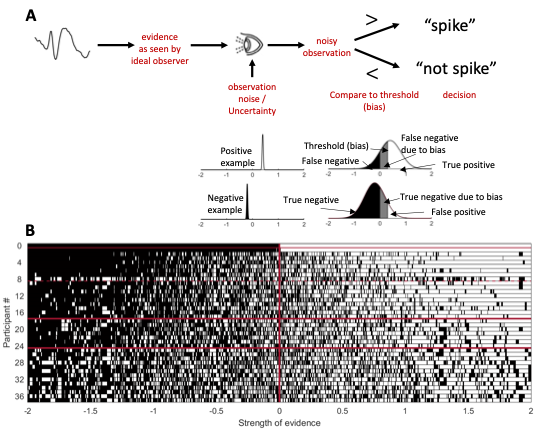
\includegraphics[width=0.75\textwidth]{Fig1-Noise-Model.png}
\caption{The LTM decision model applied to expert detection of interictal epileptiform discharges in EEG recordings. \textbf{Panel A:} Schematic of the signal detection process assumed in the LTM model. For each candidate waveform, an ideal observer would perceive the true evidence level ($c_i$). Each rater in effect receives a noisy observation ($z_{ijt} = c_i + n_{ijt}$) contaminated by perceptual or decision noise with standard deviation $\sigma_j$. The rater compares this noisy observation to their personal threshold ($\ell_j$) to produce a binary classification (IED vs. non-IED). Lower noise (higher skill $s_j = 1/\sigma_j$) produces observations closer to the true signal. \textbf{Panel B:} Heatmap showing classification decisions across 37 raters (rows) and the full range of evidence strength (columns, from strong evidence against IED on left to strong evidence for IED on right). White indicates "IED" classification; black indicates "non-IED" classification. Raters are sorted by estimated skill level (top = highest skill/lowest noise). High-skill raters show sharper transitions from black to white at consistent evidence levels, while lower-skill raters show more gradual, variable transition zones, reflecting greater noise in their decision-making.}
\label{fig:ltm-model}
\end{figure}

\begin{figure}[htbp]
\centering
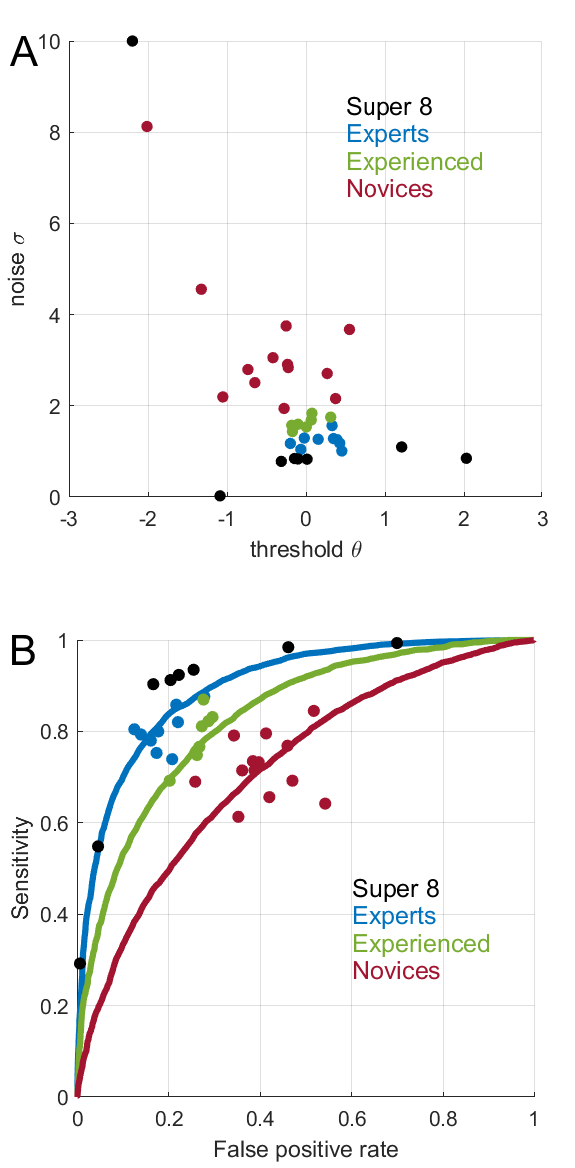
\includegraphics[width=0.5\textwidth]{SSIT-ROCs.png}
\caption{Estimated LTM parameters and resulting ROC curves by expertise level. \textbf{Panel A:} Distribution of estimated internal noise levels ($\sigma$, y-axis) and decision thresholds ($\theta$, x-axis) for each rater. Black points ('Super 8') represent 8 experts who participated in an early IED annotation study; blue points ('Experts') show additional board-certified experts who participated in a later annotation study; green points show experienced non-experts; red points show novices. Experts cluster in the low-noise region ($\sigma \approx 1$--$2$), while novices are distributed across higher noise levels ($\sigma \approx 2$--$10$). Threshold values vary across the full range for all groups, indicating that expertise affects discrimination ability (noise level) more than diagnostic bias (threshold). \textbf{Panel B:} Group-level ROC curves reconstructed from estimated parameters. Each point represents an individual rater's operating point (sensitivity vs. false positive rate). The smooth curves show the group-average ROC curves: experts (blue) achieve superior discrimination (AUC $\approx$ 0.89), experienced non-experts (green) show intermediate performance (AUC $\approx$ 0.85), and novices (red) exhibit substantially lower discrimination ability (AUC $\approx$ 0.74).}
\label{fig:ltm-roc}
\end{figure}

Grouping raters by expertise levels (Figure~\ref{fig:ltm-roc}), we see that their operating points cluster near the group-median ROC curves, suggesting that raters with similar training levels indeed have similar skill levels (Panel B). Nevertheless, decision thresholds ($\ell_j$) vary widely even among experts (Panel A), indicating that while discrimination ability is governed by level of expertise, variation in decision thresholds is a major source of between-expert disagreement for this diagnostic task. These findings show that the LTM framework successfully separates two distinct dimensions of rater performance: skill (captured by noise level $\sigma_j$, which determines the ROC curve and its AUC) and bias (captured by threshold $\ell_j$, which determines the operating point on that curve).

\subsubsection*{ROC curves, skill, and noise in the LTM}\label{section-ROC}
When working with the LTM, we assume that the correct answer $C$ for each case is available, either via an external gold standard or by taking the correct answer to be the group consensus. Each rater response can then be categorized as true positive, true negative, false positive, or false negative. We specify the percentage of positive cases ($C=1$) that the rater correctly labeled as such, known as the sensitivity $Se = Pr(Y_{ijt}=1|C=1)$, and the percentage of negative cases ($C=0$) that the rater incorrectly labeled as positive, known as the false positive rate $Fp = Pr(Y_{ijt}=1|C=0)$.

Recall that in the LTM the rater's answers $Y_{ijt}$ are determined by comparing $z_{ijt} = c_i + n_{ijt}$ with a threshold $\ell_j$. Denote the mean values of $z_{ijt}$ when $C=0$ as $\mu_0$, and the mean when $C=1$ as $\mu_1$. Assume the standard deviation of $z_{ijt}$ is $\sigma$f for both $C=1$ and for $C=1$. Then we can write the sensitivity and false positive rates as functions of $\ell_j$, $\mu_0$, $\mu_1$:
\begin{eqnarray*}
    Se(\ell_j) &=& Pr(c_{i}+n_{ijt}>\ell_j|c_{i}>0) = \Phi\left(\frac{\mu_1-\ell_j}{\sigma}\right)\\
    Fp(\ell_j) &=& Pr(c_{i}+n_{ijt}>\ell_j|c_i \leq 0) = \Phi\left(\frac{\mu_0-\ell_j}{\sigma}\right).
\end{eqnarray*}
where $\Phi$ is the standard normal cumulative distribution function. The ROC curve is the set of points $(Se, Fp)$ formed by allowing the threshold $\ell_j$ to range over all possible values. We see that each rater has a unique operating point $(Se(\ell_j), Fp(\ell_j))$ determined by their threshold. The area under the ROC curve (AUROC) is given by

$$AUROC = \Phi\left(\frac{\mu_1-\mu_0}{\sigma \sqrt{2}}\right).$$

This formulation reveals the connection between noise and discrimination: smaller $\sigma$ (higher skill) leads to higher AUROC, while the threshold $\ell_j$ determines the operating point on the ROC curve without affecting the AUROC.

\subsection*{KSS Noise decomposition}\label{section-KSS}
In the Kahneman-Sibony-Sunstein (KSS) noise decomposition framework, $$z_{ijt} = c_i + \ell_j + p_{ij} + o_{ijt},$$
where $c_i$ represents variation due to differences in case information (signal), and the other terms represent noise: $\ell_j$ is level noise, the tendency of rater $j$ to answer 'yes' or classify cases as "1" regardless of case-specific evidence; $p_{ij}$ is pattern noise, reflecting the idiosyncratic way that rater $j$ views the information in case $i$; and $o_{ijt}$ is occasion noise, reflecting differences in the response of rater $j$ to case $i$ on different occasions $t$.

Note that the total noise term $n_{ijt}$ from the LTM has been decomposed into two parts: $n_{ijt} = p_{ij} + o_{ijt}$. Each of the terms $c_i$, $\ell_j$, $p_{ij}$, $o_{ijt}$ is modeled as an independent Gaussian random variable with zero mean and standard deviations $\sigma_c$, $\sigma_\ell$, $\sigma_p$, $\sigma_o$, respectively. 

\begin{figure}[h!]
\begin{center}
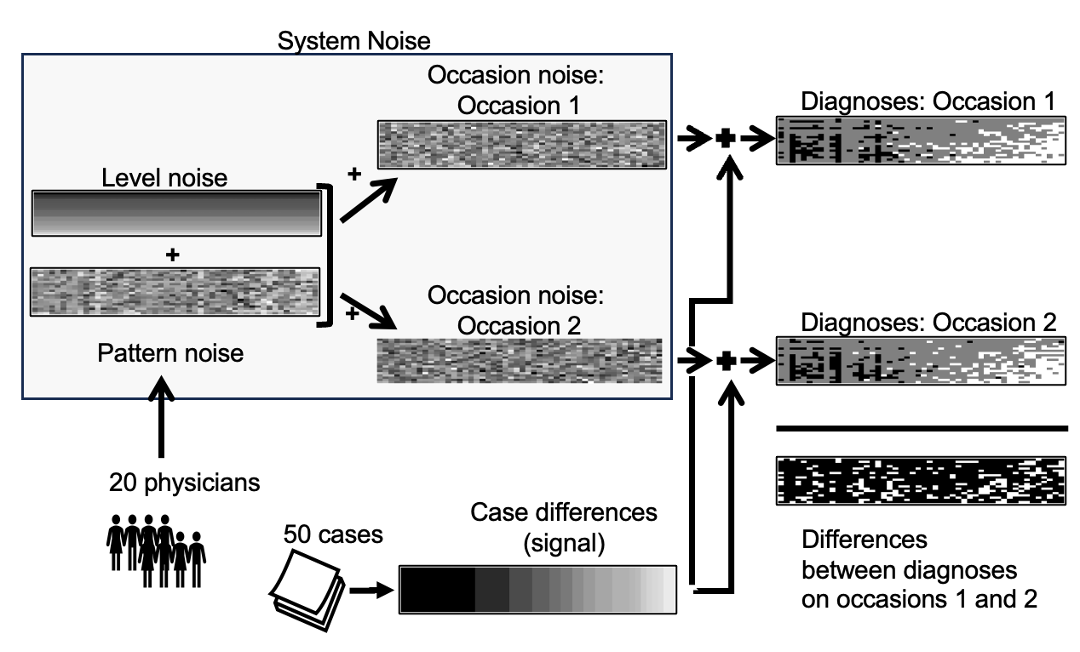
\includegraphics[width=0.70\columnwidth]{KSS-Model.png}
\caption{{\textbf{Noise decomposition: KSS framework} Illustration of how the KSS model accounts for variation in expert response data about cases histories in patients with suspected epilepsy.The three panels on the right show actual data, while the 5 on the left are estimated from the data using the KSS framework. Variation in expert responses is decomposed into signal (information intrinsic to the cases), and system noise. System noise is further decomposed into level noise, pattern noise, and occasion noise. These different types of noise are combined additively with the signal to reach a final decision. The heatmaps show the actual estimates. 
{\label{Fig3-KSS}}%
}}
\end{center}
\end{figure}

The ROC curve formulation described in the LTM section can be extended to the KSS model by treating the sum of pattern and occasion noise as total noise: $n_{ijt} = p_{ij} + o_{ijt}$, with variance $\sigma^2 = \sigma_p^2 + \sigma_o^2$. This allows computation of AUROC and rater operating points in the full KSS framework, where discrimination depends on the total noise magnitude rather than its decomposition into pattern and occasion components.

\subsection*{Unified Framework: Relating LTM and KSS}\label{section-unified}

The two models described above---LTM and KSS---are special cases of a single unified framework. Both can be expressed as generalized linear mixed models (GLMMs) with a logistic (or probit) link function:

\begin{equation}
\label{eq:master-model}
\boxed{
\begin{aligned}
Y_{ijt} &\sim \text{Bernoulli}(\pi_{ijt}) \\
\text{logit}(\pi_{ijt}) &= c_i + \ell_j + p_{ij} + o_{ijt} + \bar{y}
\end{aligned}
}
\end{equation}

where all random effects are independent and normally distributed:
$$c_i \sim \mathcal{N}(0,\sigma_c^2), \quad \ell_j \sim \mathcal{N}(0,\sigma_\ell^2), \quad p_{ij} \sim \mathcal{N}(0,\sigma_p^2), \quad o_{ijt} \sim \mathcal{N}(0,\sigma_o^2).$$

\textbf{Clinical interpretation of model components:}
\begin{itemize}
    \item $c_i$ = \textbf{Evidence in the case} (e.g., clarity of patient history, strength of EEG findings)
    \item $\ell_j$ = \textbf{Expert's personal diagnostic threshold} (tendency to over- or under-diagnose relative to peers)
    \item $p_{ij}$ = \textbf{Expert's idiosyncratic interpretation} of specific case features (stable across time)
    \item $o_{ijt}$ = \textbf{Expert inconsistency across occasions} (mood, fatigue, time of day)
    \item $\bar{y}$ = \textbf{Overall base rate} (population prevalence on logit scale)
\end{itemize}

The two models differ in how they treat discrimination noise:

\begin{itemize}
    \item \textbf{LTM:} Pattern and occasion noise are not separated; instead, $n_{ijt} = p_{ij} + o_{ijt}$ is treated as a single combined noise term with variance $\sigma^2 = \sigma_p^2 + \sigma_o^2$. This model includes case signal ($c_i$), rater thresholds ($\ell_j$), and total discrimination noise, but does not explicitly decompose noise into pattern and occasion components. The LTM is typically applied when repeated measurements (multiple occasions) are not available or when the decomposition of discrimination noise into pattern vs. occasion components is not of primary interest.

    \item \textbf{KSS (full model):} This model decomposes variation into signal ($c_i$), level noise ($\ell_j$), pattern noise ($p_{ij}$), and occasion noise ($o_{ijt}$). KSS requires repeated measurements to separate pattern noise (stable across occasions for a given rater-case pair) from occasion noise (varies across occasions).
\end{itemize}

This unified view clarifies that:
\begin{enumerate}
    \item Both models share the same underlying structure (Equation~\ref{eq:master-model})
    \item They differ only in model complexity, with KSS being more general
    \item Model selection depends on the data structure (e.g., whether repeated measurements are available) and research questions (e.g., whether separating pattern from occasion noise is important)
    \item Both models can be estimated using the same statistical framework (hierarchical Bayes or mixed-effects maximum likelihood)
\end{enumerate}

\section*{Interpretation of model parameters on the group and individual levels}\label{section-interpretation}
The KSS model is the most general of the two models, containing the LTM as a special case. Here we summarize the quantities needed to provide a full description of a set of response data within the KSS model, and their interpretation. The interpretations involve two levels: the individual and the group level.

\begin{itemize}
    \item \textbf{Individual level interpretation:}
    \begin{itemize}
    \item $c_i$ quantifies the signal, or strength of the evidence in case $i$. Larger values imply stronger evidence that the correct answer or label for case $i$ is 1, and more negative values imply stronger evidence that the correct answer is 0.
    \item $\ell_j$ quantifies the 'bias' or 'threshold' of rater $j$---the tendency to either over-call or under-call. This parameter determines the rater's operating point on a receiver-operating characteristic curve. Unlike the other parameters, $\ell_j$ represents a consistent tendency of rater $j$ that is independent of the information in any particular case $i$. From the perspective of an individual rater, this tendency is not 'noise' because it is consistent and stable across cases and occasions. However, from the perspective of the group, $\ell_j$ varies across raters and is unrelated to case-specific information; thus at the group level $\ell_j$ is noise.
    \item $p_{ij}$ quantifies pattern noise: the idiosyncratic way rater $j$ weights the information in case $i$ as favoring (when positive) or being against (when negative) labeling case $i$ as 1. For rater $j$, this response is stable across occasions: each time the rater sees case $i$, the model predicts the answer will be skewed in the same way. From the perspective of the individual rater, this tendency is not 'noise' because it is consistent across occasions. However, from the perspective of the group, $p_{ij}$ varies across raters; thus at the group level $p_{ij}$ is noise.
    \item $o_{ijt}$ quantifies the occasion noise, or variation in the response of rater $j$ to case $i$ on different occasions $t$. This quantity is considered noise at both the individual and group levels, because $o_{ijt}$ varies not only across raters but also within raters (the same rater labels the same case differently on different occasions).
    \end{itemize}
    \item \textbf{Group level interepretation:}
    \begin{itemize}
        \item $c_i$ varies across cases $i$, leading to variation in responses that is related to the underlying case information or 'signal'. This variation is modeled as $c_i \sim \mathcal{N}(0,\sigma_c^2)$.
        \item $\ell_j$ represents noise at the group level because it varies across raters $j$, independent of the underlying information $c_i$, leading the 'system' of raters to provide variable responses to the same case. This variation is modeled as $\ell_j \sim \mathcal{N}(0,\sigma_\ell^2)$.
        \item $p_{ij}$ represents noise at the group level because it varies across cases $i$ and raters $j$, independent of the underlying information $c_i$. This variation is modeled as $p_{ij} \sim \mathcal{N}(0,\sigma_p^2)$.
        \item $o_{ijt}$ represents noise at both the individual and group levels, as explained above. This variation is modeled as $o_{ijt} \sim \mathcal{N}(0,\sigma_o^2)$.
    \end{itemize}
\end{itemize}

If the number of cases is $N$, the number of raters is $M$, and the number of occasions is $T$, then the total number of responses $Y_{ijt}$ collected is $N \cdot M \cdot T$. The quantities required to fully describe the data are the actual values of the underlying variables $c_i$, $\ell_j$, $p_{ij}$, $o_{ijt}$, and the standard deviations $\sigma_c$, $\sigma_\ell$, $\sigma_p$, $\sigma_o$. Thus the total number of variables to be estimated is $N + M + N \cdot M + N \cdot M \cdot T + 4$.

All of these quantities may be of interest, or only a subset, depending on the research goals. In some cases, we may be interested only in estimating the noise magnitudes and comparing them with the signal strength; the quantities to be estimated are then $\sigma_c$, $\sigma_\ell$, $\sigma_p$, $\sigma_o$. In other cases, the aim may be to characterize the skill and decision thresholds of a group of raters with similar skill levels; the quantities of interest may be $c_i$, $\ell_j$, and the variance of the noise $\sigma$. This case is the subject of the LTM.

\section*{Identifiability and Scale}\label{section-identifiability}

Understanding the scale and identifiability of the model parameters is important for correct interpretation. This section addresses common sources of confusion.

\subsection*{The latent scale is not fully identified}

In our model, only binary outcomes $Y_{ijt} \in \{0,1\}$ are observed. The underlying latent variable $z_{ijt} = c_i + \ell_j + p_{ij} + o_{ijt} + \bar{y}$ is continuous and unobserved. Because we observe only the binary outcomes via the link function $\text{Pr}(Y_{ijt}=1) = f(z_{ijt})$, the absolute scale of the latent variable is not identified.

In the logistic model with link function $f(x) = 1/(1+\exp(-x))$, the residual variance is implicitly fixed by the link function. Specifically, the logistic distribution has variance $\pi^2/3 \approx 3.29$, which acts as an implicit scale constraint. All variance components $\sigma_c^2, \sigma_\ell^2, \sigma_p^2, \sigma_o^2$ are expressed relative to this latent scale.

In the probit model with link function $f(x) = \Phi(x)$ (standard normal CDF), the residual variance is implicitly 1. Results from logistic and probit models differ by a rescaling factor of approximately $\sqrt{\pi^2/3} \approx 1.81$.

\subsection*{Practical consequences}

\begin{enumerate}
    \item \textbf{Variance decomposition is on the latent scale.} When we report that signal accounts for X\% of total variation, this percentage is computed on the logit (or probit) scale, not on the probability scale. The latent-scale decomposition is:
    $$\text{Total Variance} = \sigma_c^2 + \sigma_\ell^2 + \sigma_p^2 + \sigma_o^2$$
    $$\text{\% Signal} = \frac{\sigma_c^2}{\sigma_c^2 + \sigma_\ell^2 + \sigma_p^2 + \sigma_o^2} \times 100$$

    \item \textbf{Variance decomposition on the probability scale requires simulation.} If you want to know "what percentage of variation in predicted probabilities is due to signal vs. noise," you must use posterior predictive simulation to compute predictions on the probability scale and then decompose their variance. This is more complex and depends on the distribution of cases (e.g., prevalence).

    \item \textbf{Absolute magnitudes of $\sigma$ values depend on the link function.} A value of $\sigma_c = 2$ in a logistic model corresponds roughly to $\sigma_c \approx 1.1$ in a probit model. However, the \textit{relative} contributions (percentages) are invariant to this rescaling.

    \item \textbf{Comparisons across studies require the same link function.} When comparing noise levels across studies, ensure both use logistic (or both use probit) links. Alternatively, report standardized effect sizes or percent contributions.

    \item \textbf{Alternative anchoring strategies.} Some researchers fix $\text{Var}(c_i) = 1$ or $\text{Var}(\ell_j) = 1$ to anchor the scale. This is a valid alternative; results differ only by rescaling. We do not adopt this approach because the logistic link provides a natural implicit anchor.
\end{enumerate}

\fbox{\begin{minipage}{0.95\textwidth}
\textbf{Key Point:} All variance components are on the latent (logit or probit) scale, not the probability scale. Percent variance contributions are interpretable and comparable within a study. For cross-study comparisons or probability-scale interpretations, use posterior predictive simulation.

\textbf{Connection to the epilepsy case study:} While we report variance components on the latent logit scale (e.g., level noise = 23\% of latent variance in Stage 1), the practical impact is seen in observable outcomes: the 16\% occasion reversal rate and 26\% inter-expert disagreement rate. The latent-scale decomposition allows us to understand \textit{why} these observable disagreements occur, but the framework's value lies in connecting abstract variance components to concrete clinical phenomena.
\end{minipage}}

\subsection*{When can one reliably estimate pattern noise?}

The pattern noise term $p_{ij}$ is a rater-by-case interaction. Estimating $\sigma_p$ requires sufficient data structure:

\begin{itemize}
    \item \textbf{Many raters AND many cases:} Pattern noise reflects how rater $j$'s response to case $i$ deviates from the additive effects of $c_i$ and $\ell_j$. To separate this interaction from residual noise, you need substantial cross-classification (many raters $\times$ many cases).

    \item \textbf{Replication helps:} If $T \geq 2$ (repeated occasions), the model can better separate pattern noise $p_{ij}$ (stable across occasions for a given rater-case pair) from occasion noise $o_{ijt}$ (varies across occasions).

    \item \textbf{With $T=1$ (single rating per rater-case pair):} The model can still estimate $\sigma_p$ via hierarchical shrinkage, but the estimate is weakly identified and relies heavily on the prior. Pattern and occasion noise in this situation are partially confounded.

\end{itemize}


\section*{Materials and Methods: Illustrative Case Study}

\subsubsection*{Case Selection and Preparation}

To demonstrate the utility of the unified framework, we applied the KSS decomposition model to diagnostic decisions from 20 board-certified epileptologists evaluating 50 clinical cases. This case study is illustrated in Figure~\ref{Fig3-KSS}. The 50 clinical cases were from adult and pediatric patients presenting with suspected seizure(s), selected from the archives of four academic tertiary epilepsy centers in the United States. To ensure a robust reference standard, all cases had an established clinical diagnosis confirmed by either (i) habitual events captured on video-EEG during an epilepsy monitoring unit (EMU) admission or (ii) a minimum of 6 months of clinical follow-up.

The case mix was intentionally balanced to represent a spectrum of case difficulty typical of a subspecialty practice:
\begin{itemize}
    \item \textbf{Prevalence:} The cohort included 25 epilepsy cases and 25 non-epilepsy cases.
    \item \textbf{Difficulty:} Cases were categorized by the authors into four difficulty bins (easy, moderate, difficult, and very difficult) to ensure a broad spectrum of diagnostic complexity.
    \item \textbf{Case Profiles:} Among epilepsy cases, 12 were confirmed by EEG and 13 by follow-up; among non-epilepsy cases, 6 were confirmed by EEG and 19 by follow-up.
\end{itemize}

\subsubsection*{Participants and Experimental Procedure}

Twenty board-certified multinational epileptologists from 18 academic centers across 5 countries were recruited to independently review the cases. Experts had an average of 20 years in practice (range: 2.5-40 years; median: 19 years). The experiment followed a three-step structured judgment process:

\begin{enumerate}
    \item \textbf{Initial Assessment (Question 1):} Experts reviewed a clinical vignette summarizing history and physical exam data and rated the likelihood of epilepsy as "low," "intermediate," or "high".

    \item \textbf{Supplemental Testing (Question 2):} If "intermediate" was selected, experts were provided with a representative 10- to 20-second routine scalp EEG epoch and a summary of neuroimaging findings. They then provided a binary "yes/no" diagnosis.

    \item \textbf{Difficulty Rating (Question 3):} Experts rated the perceived difficulty of each case using a 5-point Likert scale.
\end{enumerate}

To measure occasion noise, the entire process was repeated after a washout period of at least 30 days.


\subsubsection*{Response Coding for Variance Decomposition}

For the noise decomposition analysis, we modeled responses to both questions as binary outcomes. For Question 1, we coded "high" probability (the expert believes the patient has epilepsy) as 1, while both "low" and "intermediate" were coded as 0. For Question 2, the responses were already binary ("yes" = 1, "no" = 0). This coding scheme allows us to apply the unified GLMM framework (Equation~\ref{eq:master-model}) to decompose variance into signal and noise components separately for each diagnostic stage.

\subsection*{Results}

\subsubsection*{Variability and Consistency}

Experts varied widely in their diagnostic thresholds and interpretations. The probability of receiving a different final diagnosis when seeing the same expert on different occasions was 16\% (162 diagnostic reversals out of 1,000 case evaluations). The probability of two different experts making a different diagnosis for the same case was 26\%. At the individual case level, the proportion of experts diagnosing epilepsy ranged from 0\% to 80\% across the 50 cases, with the number of experts requesting supplemental testing (EEG/neuroimaging) ranging from 4 to 20 per case.

\subsubsection*{Noise Decomposition}

\textbf{A Shift in Noise Profiles.} We applied the KSS model (Equation~\ref{eq:master-model}) to decompose variation in expert diagnoses. The framework reveals a fundamental shift in the source of disagreement when experts move from clinical history alone to a full diagnostic workup. Table~\ref{tab:variance-results} summarizes the variance components for both stages.

\begin{table}[h!]
\centering
\small
\begin{tabular}{lcccc}
\toprule
& \multicolumn{2}{c}{\textbf{Question 1 (History Only)}} & \multicolumn{2}{c}{\textbf{Question 2 (Final Diagnosis)}} \\
\cmidrule(lr){2-3} \cmidrule(lr){4-5}
\textbf{Component} & \textbf{Std. Dev ($\sigma$)} & \textbf{\% Variation} & \textbf{Std. Dev ($\sigma$)} & \textbf{\% Variation} \\
\midrule
\textbf{Signal ($c_i$)} & -- & 66\% & -- & 69\%  \\
\textbf{Level Noise ($\ell_j$)} & -- & 23\% & -- & 5\%  \\
\textbf{Pattern Noise ($p_{ij}$)} & -- & 10\% & -- & 24\%  \\
\textbf{Occasion Noise ($o_{ijt}$)} & -- & 1\% & -- & 1\%  \\
\midrule
\textbf{Total System Noise} & -- & 34\% & -- & 31\%  \\
\bottomrule
\end{tabular}
\caption{Variance decomposition of expert responses in epilepsy diagnosis. Percentages represent the proportion of total variation explained by each component on the latent (logit) scale. Question 1 was based on clinical history alone; Question 2 incorporated EEG and neuroimaging results.}
\label{tab:variance-results}
\end{table}

\textbf{Stage 1 (Clinical History Only):} Disagreement was primarily driven by \textit{level noise} (23\% of total variation). This suggests that in the absence of objective data, expert disagreement is a "threshold problem"---some experts are simply more inclined to diagnose epilepsy than others. 

\textbf{Stage 2 (Full Diagnostic Workup):} Once EEG and neuroimaging data were introduced, level noise decreased to 5\%, but \textbf{pattern noise} rose to 24\%. This indicates that supplemental testing "calibrates" experts' thresholds (reducing systematic bias) but introduces new idiosyncratic disagreements regarding the interpretation of specific test features. 

\textbf{Key findings from the variance decomposition:}

\begin{itemize}
    \item \textbf{Noise Magnitude:} Approximately one-third of the total variation in final expert diagnoses was attributable to noise (31-34\%).

    \item \textbf{The "Information Shift":} Providing additional diagnostic information (EEG/neuroimaging) reduced overall noise only modestly (from 34\% to 31\%), but \textit{shifted the dominant noise source}. The framework reveals that moving from subjective to objective data does not eliminate disagreement---it transforms it from a threshold problem (level noise) to an interpretation problem (pattern noise).

    \item \textbf{Expert Inconsistency:} While the probability of an expert disagreeing with their own previous diagnosis was 16\%, occasion noise only accounted for 1\% of the total variance. This suggests that diagnostic "flip-flopping" happens mostly when cases are inherently ambiguous or near the expert's decision threshold. 

    \item \textbf{Difficulty Impact:} Most noise and disagreement occurred in "difficult" cases, where expert agreement dropped to 50\%.
\end{itemize}

Figure~\ref{fig:variance-decomp} visualizes the variance decomposition across all three diagnostic stages. The Gaussian distributions illustrate the estimated magnitude of each variance component (signal and noise types), with tick marks showing the distribution of estimated random effects. The stacked bar charts quantify the relative contribution of each component to total variation. The dramatic shift in noise profile from Stage 1 to Stage 2 is immediately apparent: level noise (medium gray) shrinks from 23\% to 5\%, while pattern noise (light gray) expands from 10\% to 24\%, despite total system noise remaining nearly constant at approximately one-third of total variation.

\begin{figure}[h!]
\centering
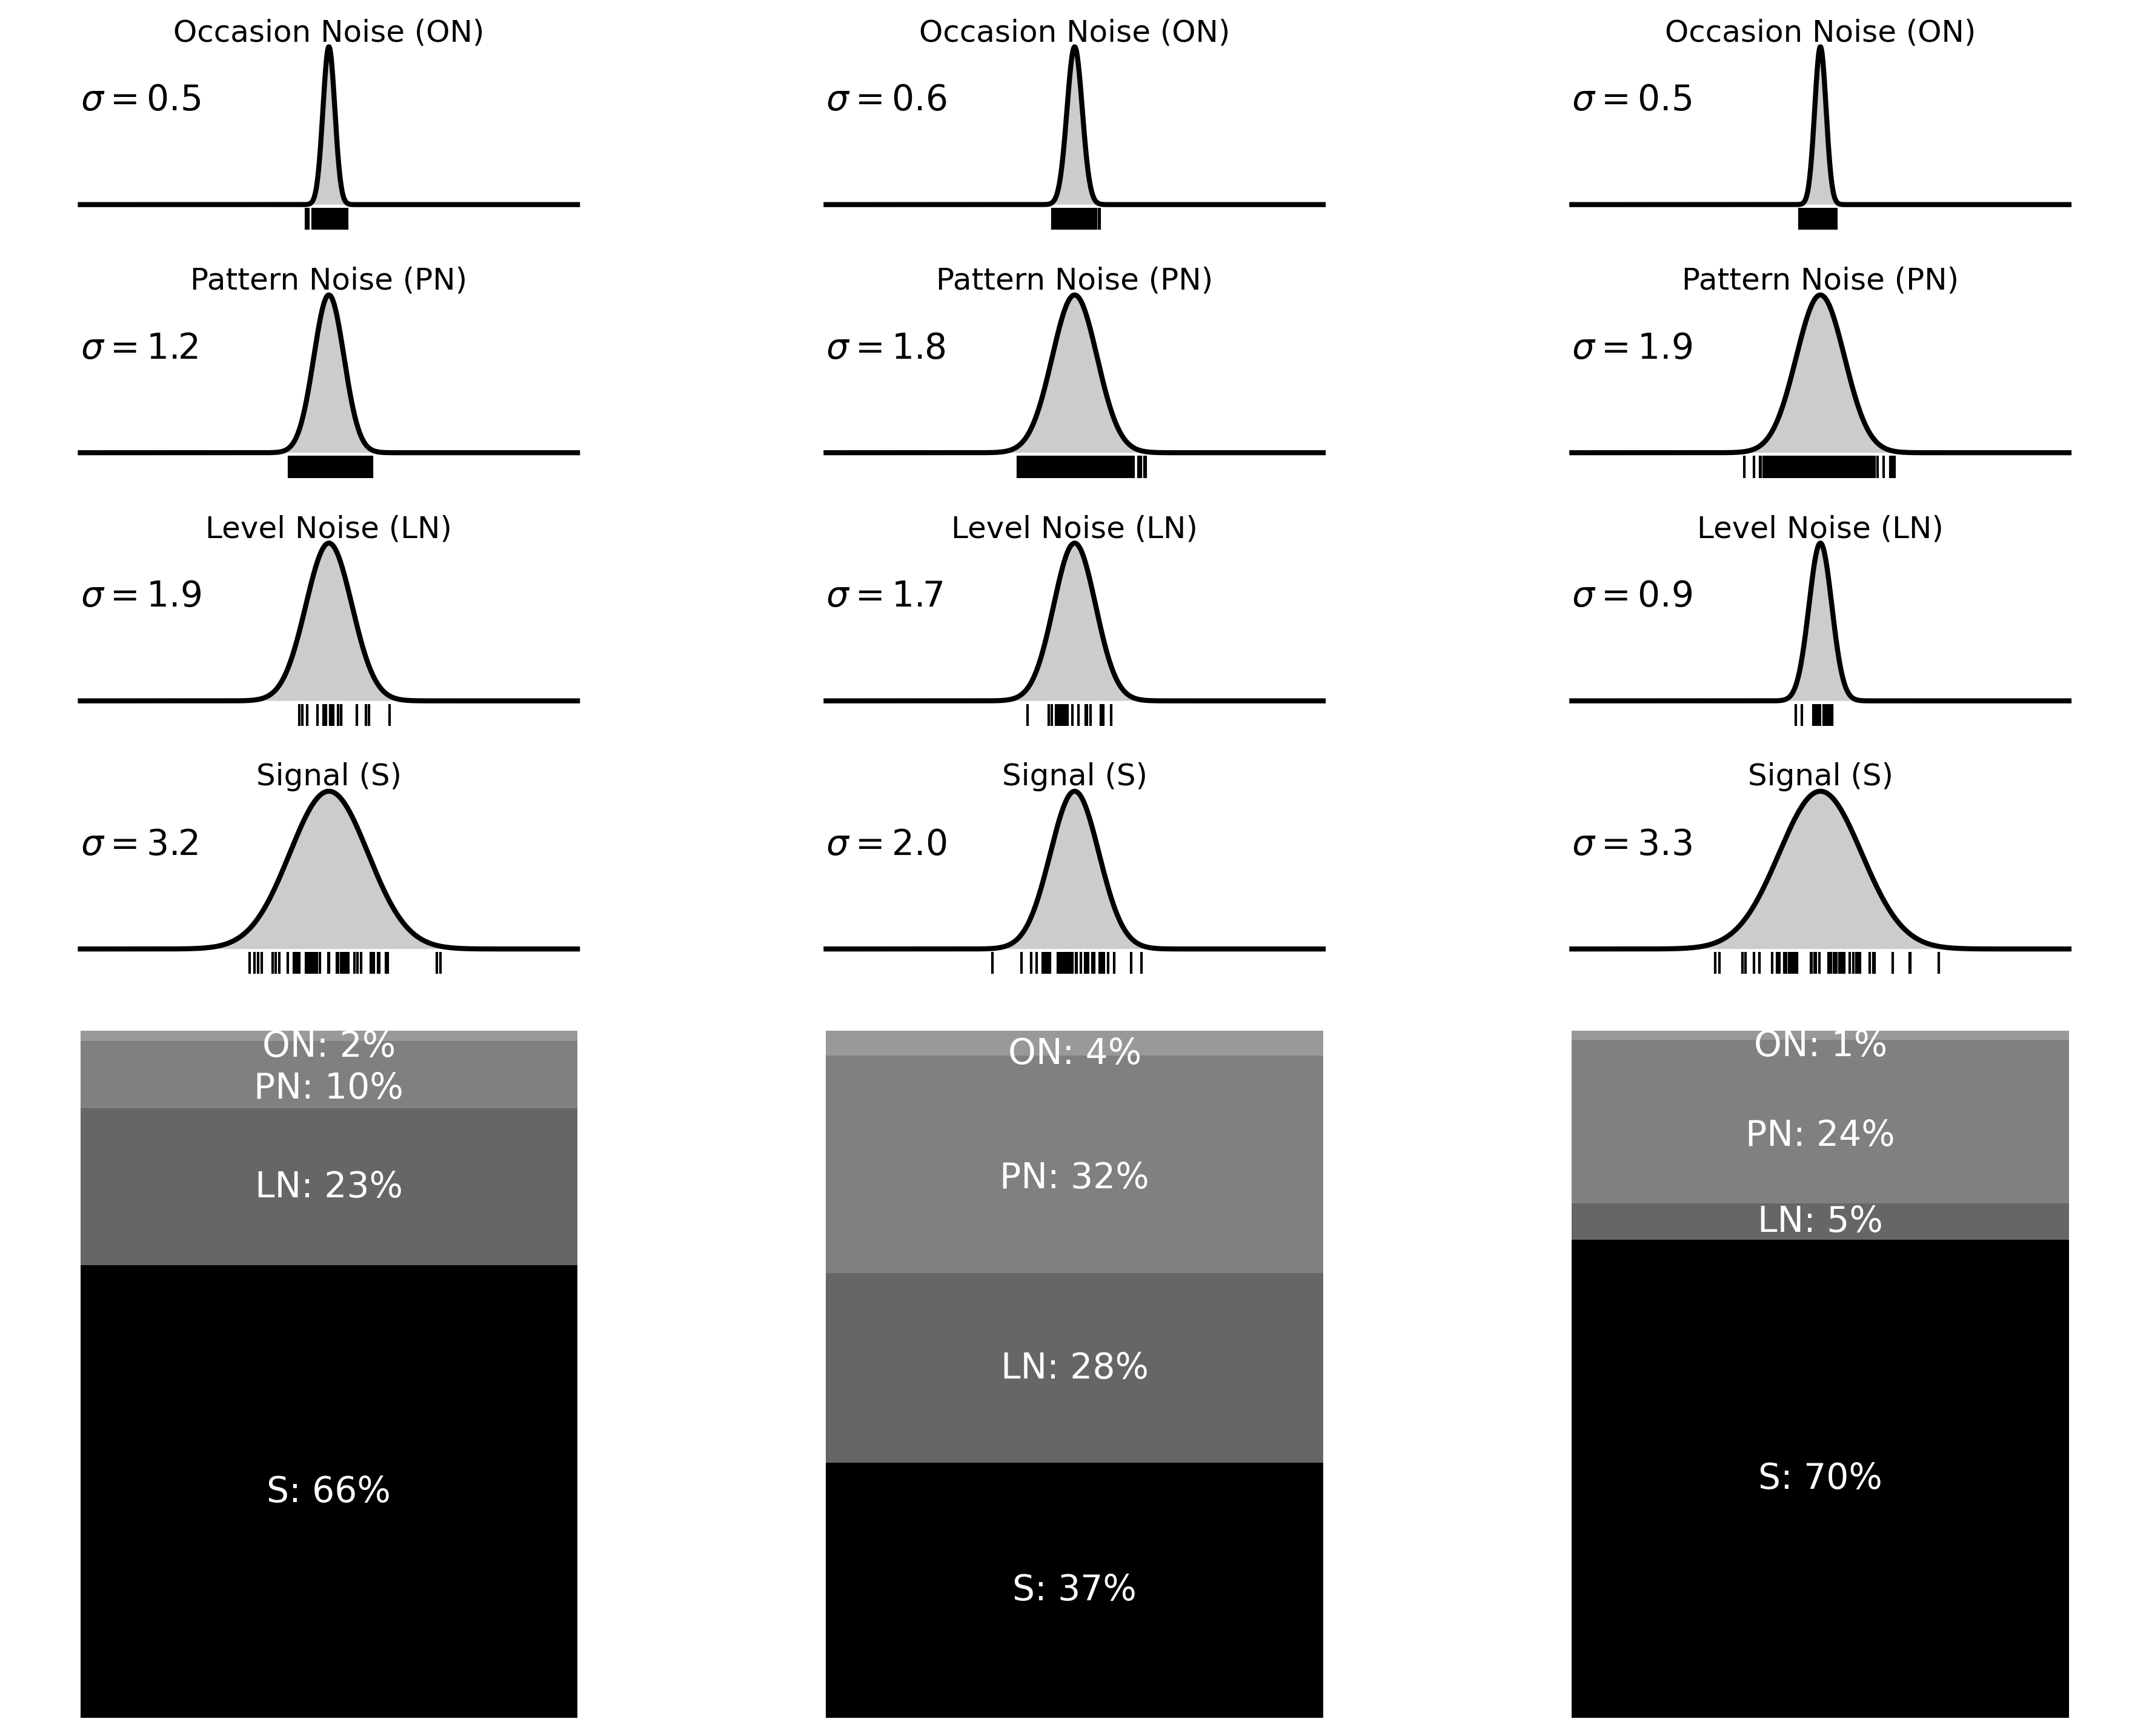
\includegraphics[width=0.95\textwidth]{Figure3.png}
\caption{Variance decomposition across three diagnostic stages in the epilepsy case study. Each column represents a different diagnostic stage: \textbf{Left:} Stage 1 (clinical history only); \textbf{Middle:} Decision to request supplemental testing; \textbf{Right:} Stage 2 (final diagnosis with EEG and neuroimaging). For each stage, Gaussian curves show the distribution of estimated variance components, with tick marks indicating individual random effect estimates. Stacked bar charts (bottom) display percentage contributions to total variation. S = signal (case difficulty); LN = level noise (systematic expert threshold differences); PN = pattern noise (idiosyncratic case interpretation); ON = occasion noise (within-expert inconsistency). Note the "information shift": adding objective tests (Stage 1 to Stage 2) reduces level noise (23\% $\rightarrow$ 5\%) but increases pattern noise (10\% $\rightarrow$ 24\%), transforming disagreement from a threshold problem to an interpretation problem.}
\label{fig:variance-decomp}
\end{figure}

\subsubsection*{Diagnostic Accuracy}

Mean accuracy relative to the clinical diagnosis was 60\% after Question 1 (range across experts: 50-70\%) and 71\% after the final diagnosis incorporating test results (range: 63-81\%). Accuracy varied substantially with case difficulty. For cases rated as easy or moderate by study authors, mean accuracy was 87\%, while for difficult and very difficult cases, accuracy dropped to 56\%. Among cases rated as easy by experts during the study, mean accuracy was 92\%, whereas cases rated as neither easy nor difficult had mean accuracy of 64\%.

Notably, diagnostic accuracy did not significantly correlate with years of practice (r = 0.18, p = 0.46), suggesting that experience alone does not eliminate noise. This underscores the need for systematic approaches to improve diagnostic reliability beyond simply accumulating clinical experience. 

\subsection*{Intervention Roadmap: From Measurement to Action}

The primary value of decomposing noise into distinct types is that each suggests different remedies. Table~\ref{tab:intervention-roadmap} maps the mathematical output of the model to specific quality improvement actions.

\begin{table}[h]
\centering
\caption{Intervention roadmap: Mapping noise types to targeted quality improvement strategies}
\label{tab:intervention-roadmap}
\begin{tabular}{@{}p{0.2\textwidth}p{0.3\textwidth}p{0.4\textwidth}@{}}
\toprule
\textbf{If the model shows high...} & \textbf{It means...} & \textbf{Recommended Intervention} \\
\midrule
\textbf{Level Noise} ($\sigma_\ell^2$) &
Experts have systematically different diagnostic thresholds (some are more conservative, others more liberal). &
\begin{itemize}[leftmargin=*, nosep]
    \item Threshold calibration exercises with known-difficulty cases
    \item Standardized diagnostic guidelines with explicit criteria
    \item Feedback on personal diagnostic tendencies
\end{itemize} \\
\midrule
\textbf{Pattern Noise} ($\sigma_p^2$) &
Experts interpret the same case features differently (e.g., disagreement on what constitutes a "significant" EEG spike). &
\begin{itemize}[leftmargin=*, nosep]
    \item Case-based group training sessions with discussion of discordant cases
    \item AI-assisted feature detection to standardize measurements
    \item Develop shared mental models through deliberate practice
\end{itemize} \\
\midrule
\textbf{Occasion Noise} ($\sigma_o^2$) &
Individual experts are inconsistent over time (fatigue, mood, time-of-day effects). &
\begin{itemize}[leftmargin=*, nosep]
    \item Decision support tools that prompt consistency checks
    \item "Second-read" protocols for borderline cases
    \item Workflow scheduling to minimize fatigue effects
\end{itemize} \\
\bottomrule
\end{tabular}
\end{table}

\subsection*{Interpreting the Shift: A Guide for Quality Improvement}

The epilepsy case study illustrates why traditional reliability metrics are insufficient for guiding interventions. A conventional analysis using Cohen's kappa would show modest improvement in agreement from Stage 1 to Stage 2, leading to the conclusion that "adding EEG and neuroimaging improves diagnostic reliability." While technically true, this misses the actionable insight.

\textbf{What traditional metrics would show:}
\begin{itemize}
    \item Stage 1 (History): Fair agreement (Fleiss' kappa = 0.33)
    \item Stage 2 (History + EEG/Imaging): Moderate agreement (Fleiss' kappa = 0.52)
    \item Conclusion: "EEG improves reliability"
\end{itemize}

However, these summary statistics conceal substantial heterogeneity. Pairwise Cohen's kappa between individual expert pairs ranged from $-0.06$ to $1.00$ in Stage 1 (mean = 0.27, SD = 0.27) and from $0.09$ to $0.84$ in Stage 2 (mean = 0.52, SD = 0.14). The dramatic reduction in variability (SD decreased by nearly half) indicates that objective testing not only improves average agreement, but also reduces the dispersion of agreement across expert pairs---some pairs of experts who strongly disagreed on clinical history alone achieved moderate agreement once test results were available.

\textbf{What the noise decomposition reveals:}
\begin{itemize}
    \item Stage 1: The disagreement is primarily a \textbf{Rater Problem} (Level Noise = 23\%). Different experts have different thresholds for what constitutes "sufficient evidence" for epilepsy diagnosis.
    \item Stage 2: The disagreement transforms into a \textbf{Feature Interpretation Problem} (Pattern Noise = 24\%). Experts now agree on general thresholds, but disagree on how to interpret specific EEG morphologies or imaging findings.
\end{itemize}

\textbf{Implications for quality improvement:}
\begin{itemize}
    \item \textit{Wrong intervention:} A quality improvement team using only kappa might conclude "we need more testing" or "we need better tests."
    \item \textit{Correct intervention:} The framework reveals that Stage 1 requires \textbf{threshold calibration} (e.g., anchoring vignettes, consensus guidelines on diagnostic thresholds), while Stage 2 requires \textbf{feature standardization} (e.g., EEG morphology atlases, inter-rater training on spike classification, AI-assisted feature detection).
\end{itemize}

This is the core value proposition of the framework: it transforms reliability measurement from a descriptive statistic into a diagnostic tool that identifies \textit{which} intervention will be most effective at each stage of the diagnostic process.


\section*{Model Validation: Posterior Predictive Checks}\label{section-ppc}

Model validation is essential to ensure that the fitted model adequately captures the structure of the observed data. We recommend the following posterior predictive checks, which we illustrate using results from the epilepsy case study (Stage 2: History + EEG/Imaging data):

\subsection*{Check 1: Case-Level Agreement}

For each case $i$, compute:
\begin{itemize}
    \item Observed proportion of "yes" responses: $\bar{y}_i^{\text{obs}}$
    \item Predicted proportion from posterior: $\bar{y}_i^{\text{pred}}$
\end{itemize}
Plot observed vs. predicted. Points should cluster along the diagonal $y = x$.

\subsection*{Check 2: Rater-Level Positive Rates}

For each rater $j$:
\begin{itemize}
    \item Observed positive rate: $\bar{y}_j^{\text{obs}}$
    \item Predicted positive rate: $\bar{y}_j^{\text{pred}}$
\end{itemize}
Plot observed vs. predicted. This checks whether the model captures individual rater biases ($\ell_j$).

\subsection*{Check 3: Switch Rates (if T $\geq$ 2)}

For rater-case pairs rated on multiple occasions:
\begin{itemize}
    \item Observed switch rate: \% of cases where rater changed answer
    \item Predicted switch rate from posterior samples
\end{itemize}
Compare distributions. This validates the occasion noise component ($\sigma_o$).

\subsection*{Check 4: Heatmap Comparison}

Generate heatmaps of:
\begin{itemize}
    \item Observed responses $Y_{ij}$ (cases × raters)
    \item Replicated data from posterior predictive distribution
\end{itemize}
Visual similarity confirms that the model captures the overall pattern structure.

\subsection*{Validation Results: Epilepsy Case Study}

We applied these posterior predictive checks to validate model fit for the epilepsy diagnosis data. Results demonstrate excellent model performance across all checks:

\textbf{Check 1 (Case-Level Agreement):} The correlation between observed and predicted proportions of affirmative diagnoses across 50 cases was $r = 0.999$, with mean absolute error of 0.025. Points clustered tightly along the diagonal, indicating the model accurately captures case-level difficulty.

\textbf{Check 2 (Rater-Level Positive Rates):} The correlation between observed and predicted diagnostic rates across 20 experts was $r = 0.998$, with mean absolute error of 0.009. This confirms that the model successfully captures systematic differences in expert diagnostic thresholds (the level noise component).

\textbf{Check 3 (Switch Rates):} The observed diagnostic reversal rate between occasions was 16.2\%, consistent with the reported occasion noise component. Despite occasion noise contributing only 1\% to total variance, this small component is sufficient to produce observable within-expert inconsistency for cases near an expert's decision threshold.

These validation results confirm that the hierarchical GLMM framework provides an appropriate statistical model for the observed diagnostic patterns, successfully decomposing variation into interpretable signal and noise components (Figure~\ref{fig:ppc}).

\begin{figure}[h!]
\centering
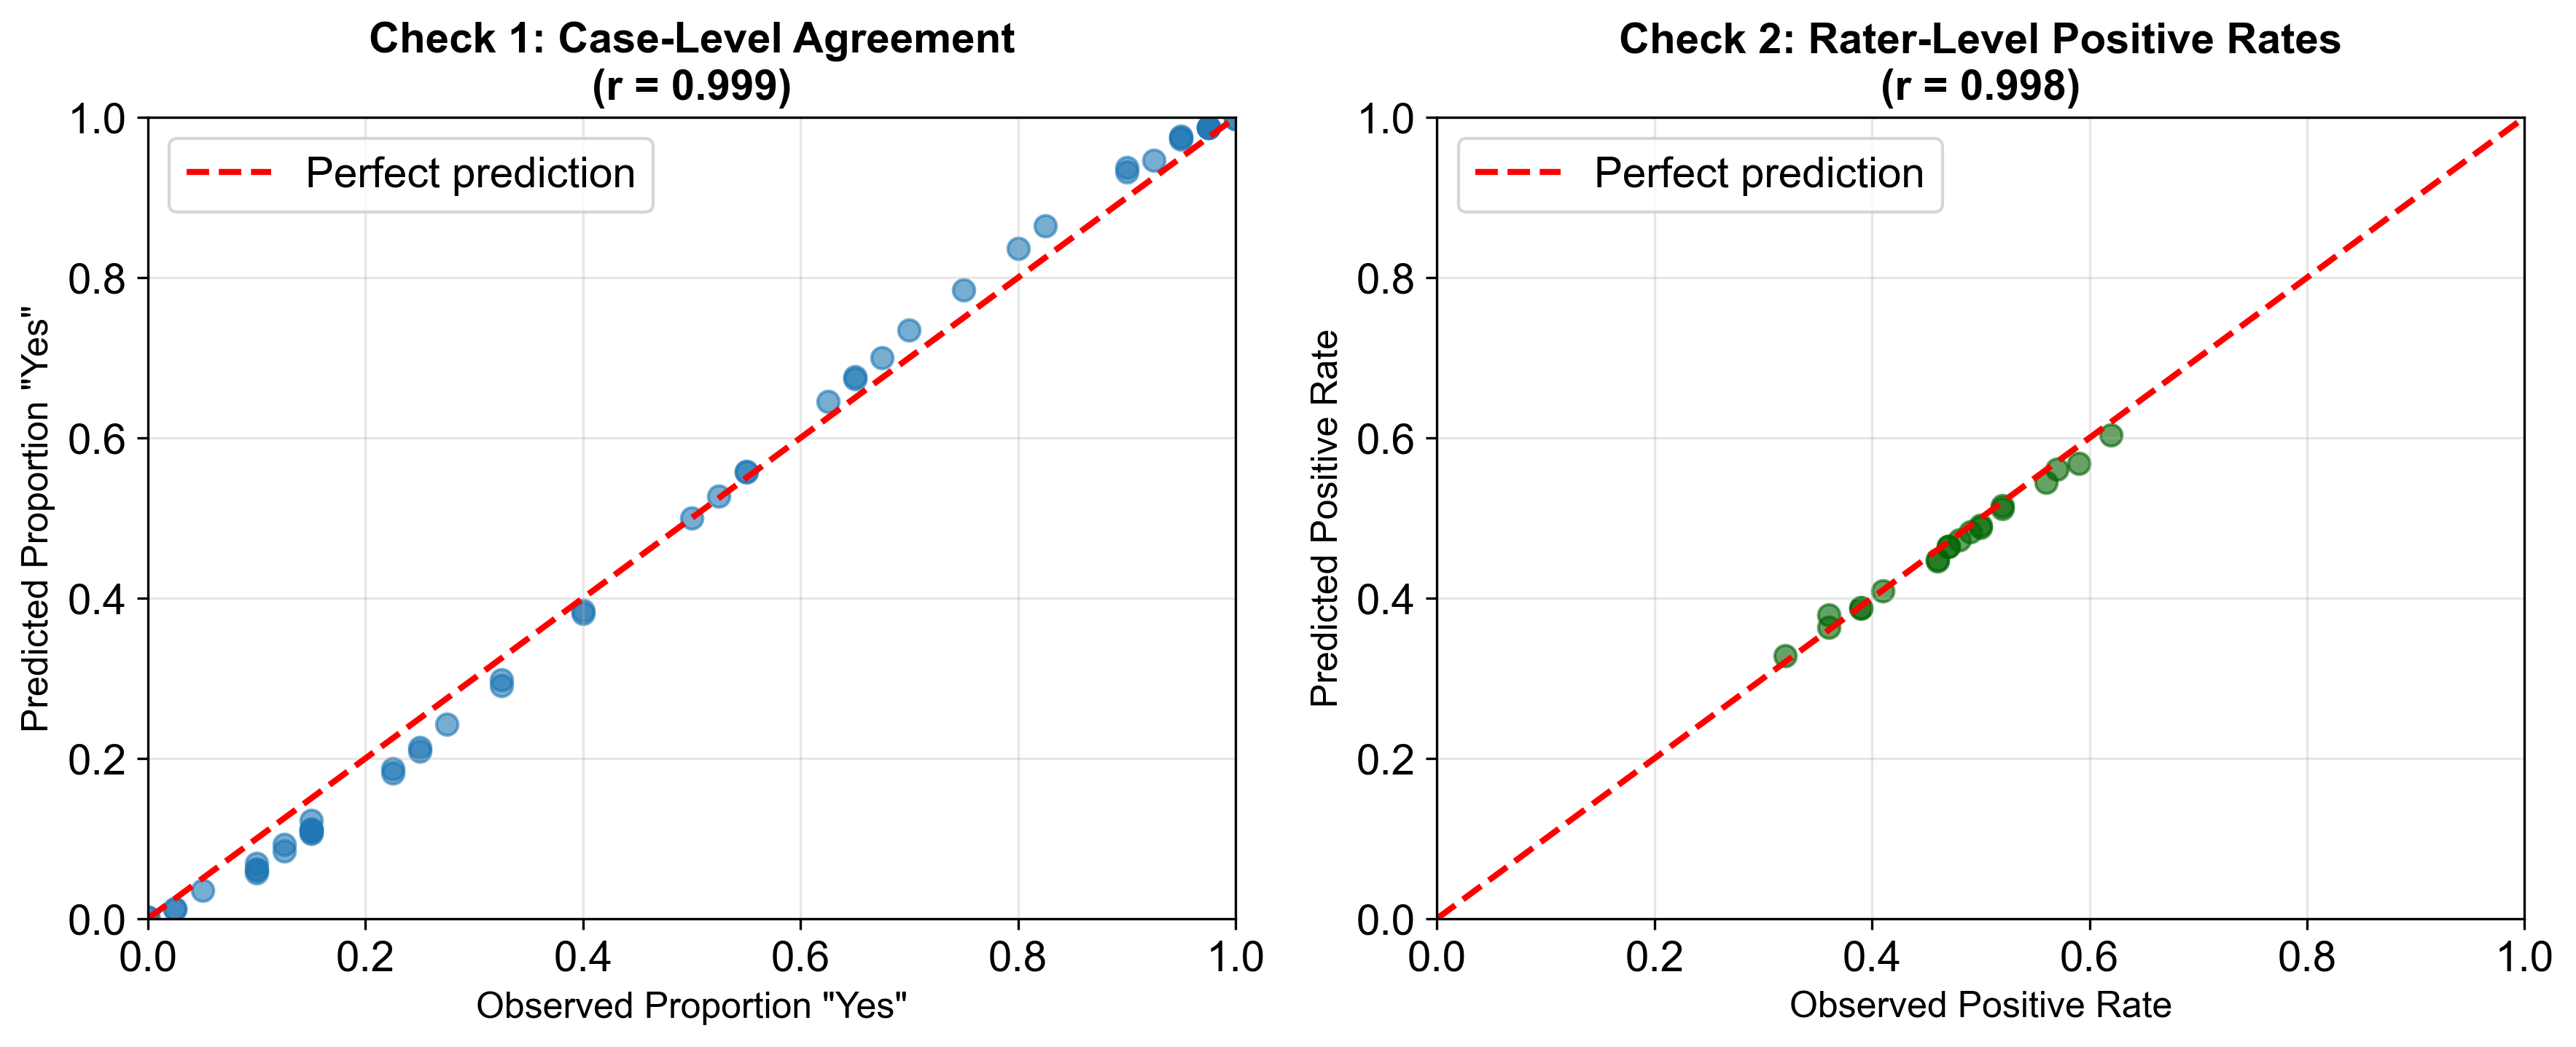
\includegraphics[width=0.95\textwidth]{posterior_predictive_checks.png}
\caption{Posterior predictive checks for model validation. \textbf{Left panel:} Case-level agreement showing observed versus predicted proportion of affirmative diagnoses across 50 cases ($r = 0.999$). \textbf{Right panel:} Rater-level positive rates showing observed versus predicted diagnostic rates across 20 experts ($r = 0.998$). Points cluster tightly along the diagonal (red dashed line) in both panels, confirming excellent model fit.}
\label{fig:ppc}
\end{figure}

\section*{Discussion}

Reliability in expert judgment is not a single number---it is a system property with multiple failure modes. Traditional metrics such as Cohen's kappa or the intraclass correlation coefficient quantify \textit{how much} experts disagree, but not \textit{why}. A kappa of 0.65 indicates moderate agreement, yet provides no insight into whether disagreement stems from misaligned diagnostic thresholds, idiosyncratic interpretation of clinical features, or temporal inconsistency within individual raters. Each of these sources requires fundamentally different interventions.

The unified framework presented here addresses this limitation by decomposing total disagreement into actionable variance components: level noise ($\sigma_\ell^2$) quantifies systematic threshold differences across raters; pattern noise ($\sigma_p^2$) captures idiosyncratic interpretation of specific cases; and occasion noise ($\sigma_o^2$) measures within-rater inconsistency over time. This decomposition is not merely descriptive---it directly informs targeted quality improvement strategies, as detailed in the intervention roadmap (Table~\ref{tab:intervention-roadmap}).

\subsection*{Relationship to Existing Reliability Metrics}

Our approach builds upon and extends traditional reliability frameworks. Cohen's kappa and Fleiss' kappa provide useful baseline measures of overall agreement, but do not partition disagreement into specific sources \cite{Kahneman2021}. We recommend reporting kappa alongside noise decomposition: kappa quantifies the magnitude of the problem, while variance components identify which interventions will be most effective. 

The intraclass correlation coefficient (ICC) corresponds to the signal-to-total-variance ratio in our framework: $\sigma_c^2 / (\sigma_c^2 + \sigma_\ell^2 + \sigma_p^2 + \sigma_o^2)$. While ICC is appropriate when only total reliability matters, quality improvement requires knowing whether the remaining variation arises from systematic bias (level noise), idiosyncratic interpretation (pattern noise), or random inconsistency (occasion noise).

Generalizability theory (G-theory) \cite{Cronbach1972,Brennan2001,Shavelson1991} is the closest conceptual relative to our framework. Both approaches decompose variance into multiple facets. However, classical G-theory relies on ANOVA-based methods appropriate for continuous outcomes, whereas medical decisions are typically binary. Our framework uses generalized linear mixed models (GLMMs) to extend G-theory to binary data \cite{Jiang2018}, while maintaining explicit connections to signal detection theory and item response theory. The correspondence is direct: the G-theory "universe score" maps to our case signal ($c_i$), the "rater facet" corresponds to level noise ($\ell_j$), the "rater $\times$ item interaction" corresponds to pattern noise ($p_{ij}$), and the "residual" corresponds to occasion noise ($o_{ijt}$).

\subsection*{Practical Implications: The Information Shift}

The epilepsy case study illustrates why decomposition matters for quality improvement. When experts moved from clinical history alone to a full diagnostic workup including EEG and neuroimaging, traditional metrics showed modest improvement (kappa increased from 0.33 to 0.52). This would suggest the intervention worked. However, the variance decomposition revealed that total noise barely changed (34\% to 31\%), but the \textit{source} of disagreement fundamentally shifted: level noise decreased from 23\% to 5\%, while pattern noise increased from 10\% to 24\%.

This "information shift" demonstrates that adding objective diagnostic tests does not eliminate disagreement---it transforms the problem from threshold miscalibration to feature interpretation. Without noise decomposition, quality improvement teams might conclude that "more testing" improves reliability and pursue further test development. The variance components reveal a different prescription: Stage 1 requires threshold calibration (e.g., consensus guidelines on diagnostic criteria), whereas Stage 2 requires feature standardization (e.g., training on EEG morphology interpretation, potentially supplemented by AI-assisted feature detection).

\subsection*{Methodological Contributions}

This framework unifies three previously separate reliability paradigms---item response theory, social signal interpretation theory, and the Kahneman-Sibony-Sunstein noise framework---as special cases of a single generalized linear mixed model (Equation~\ref{eq:master-model}). This unification provides a common statistical foundation for measuring reliability across diverse domains, from radiology to psychiatry to forensic science.

The Bayesian implementation offers additional advantages. Uncertainty quantification through posterior distributions enables principled comparison of variance components, while hierarchical shrinkage provides stable estimates even with modest sample sizes. Posterior predictive checks validate model assumptions by comparing observed data patterns to model-generated predictions.

\subsection*{Limitations and Future Directions}

Several limitations warrant consideration. First, the framework assumes that disagreement can be meaningfully partitioned into the three noise types. In practice, these components may interact in complex ways not captured by the additive variance structure. Second, the binary outcome model may oversimplify clinical judgment when diagnostic confidence varies continuously. Extensions to ordinal or continuous outcomes would broaden applicability.

Third, our case study involved a selected set of cases evaluated under controlled experimental conditions. Real-world diagnostic reliability may differ due to factors such as time pressure, incomplete information, or variations in case presentation format. Prospective studies embedding noise audits into routine clinical workflows would provide more ecologically valid estimates.

Fourth, while we demonstrated the framework in epilepsy diagnosis, validation across diverse medical specialties is needed. Different domains may exhibit different noise profiles, and the optimal intervention strategies may vary accordingly. We encourage researchers to apply this framework to their own reliability studies and contribute to a growing evidence base on domain-specific noise patterns.

Finally, the framework identifies sources of disagreement but does not directly address whether any particular expert judgment is correct. High agreement does not guarantee accuracy if all experts share the same systematic bias. Future work should integrate noise decomposition with measures of calibration against established reference standards.

\subsection*{Conclusions}

For researchers seeking to improve expert consensus in medical diagnosis, the relevant question is not "How reliable are my experts?" but rather "What type of unreliability do I have, and what intervention will address it?" This framework provides both the measurement tool and the intervention roadmap to answer that question. By transforming reliability measurement from a descriptive statistic into a diagnostic instrument, variance decomposition enables evidence-based quality improvement in expert judgment.


% Appendices
\section*{Appendix A: Bayesian Estimation Details}\label{section-estimation}

The observed expert responses $y_{ijt}$ are binary (yes/no), while the underlying (unobserved) signal and noise are continuous, requiring a statistical approach to estimate the variance components $\sigma_c$, $\sigma_\ell$, $\sigma_p$, $\sigma_o$ from the observations.

The model is a generalized linear mixed-effects model (GLMM). The underlying parameter values that must be estimated include the random effects $c_j$, $\ell_i$, $p_{ij}$, $o_{ijt}$, $\bar{y}$, and their standard deviations, $\sigma_c$, $\sigma_\ell$, $\sigma_p$, $\sigma_o$.

\subsection*{Why Bayesian estimation?}
Because of the nonlinearity of the logistic link function, the marginal likelihood (obtained by integrating out the latent variables) is analytically intractable. While maximum likelihood estimation via Laplace approximation is possible using standard software (e.g., \texttt{lme4} in R, \texttt{glmmTMB}), we adopt a fully Bayesian approach using Markov chain Monte Carlo (MCMC) sampling because it provides full posterior distributions for all parameters (enabling proper uncertainty quantification), handles the complex hierarchical structure without approximation, allows for flexible prior specification to improve identifiability, and enables posterior predictive checks for model validation.

\subsection*{Implementation details}
We place weakly informative half-normal priors on the variance parameters $\sigma_c$, $\sigma_\ell$, $\sigma_p$, and $\sigma_o$. To improve MCMC sampling efficiency in this hierarchical model, we adopt a non-centered parameterization. For example, the case effect is reparameterized as $z_{c,j} \sim \mathcal{N}(0,1)$ and $c_j = \sigma_c z_{c,j}$, with analogous formulations for $\ell_i$, $p_{ij}$, and $o_{ijt}$. This reparameterization addresses the funnel-shaped geometry common in hierarchical models and improves sampling efficiency.

We employ the No-U-Turn Sampler (NUTS) as implemented in PyMC with NumPyro backend. Our sampling configuration uses 4 parallel chains, 2,000 tuning (warmup) iterations per chain, 2,000 post-tuning draws per chain, and a target acceptance rate of 0.98.

Convergence is assessed using standard diagnostics: $\hat{R}$ statistics (should be $<1.01$), effective sample size (should be $>400$ per chain), and visual inspection of trace plots.

\textbf{Computational considerations.} The full KSS model scales with the number of case--rater--occasion combinations (approximately $O(N \times M \times T)$). For very large studies, computational burden may motivate fitting reduced models (e.g., LTM with a single combined noise term) or restricting repeated measurements to a subset of cases or raters. These simplifications preserve the core signal--noise separation while improving scalability.

\subsection*{Variance decomposition from posterior samples}
After obtaining the posterior distributions, we compute posterior means and credible intervals for the standard deviation parameters. The percentage of total variance explained by each component is:
\begin{eqnarray*}
\text{\% Component} = \frac{\sigma^2_{\text{component}}}{\sigma^2_c + \sigma^2_\ell + \sigma^2_p + \sigma^2_o} \times 100
\end{eqnarray*}
Credible intervals for these percentages are computed from the posterior samples.

The accompanying GitHub repository contains the \textbf{reference implementation} used to generate all figures, tables, and analyses reported in this manuscript, including data preprocessing, model fitting, posterior predictive checks, and figure generation. The code snippets in this appendix are illustrative; the repository provides the complete, versioned workflow: (GITHUB LINK).


\section*{Appendix B: How to Use This Method in Practice}\label{section-practical-guide}

This section provides step-by-step guidance for applied researchers on implementing the noise decomposition framework.

\subsection*{Step 1: Prepare the Response Matrix}

Organize your data as a three-dimensional array (or long-format data frame):
\begin{itemize}
    \item \textbf{Cases (i):} Rows represent distinct cases, patients, or items to be rated
    \item \textbf{Raters (j):} Columns represent individual raters or experts
    \item \textbf{Occasions (t):} If available, include repeated ratings of the same case by the same rater
    \item \textbf{Missing data:} The Bayesian framework handles missing data naturally; not all raters need to rate all cases
\end{itemize}

\subsection*{Step 2: Choose Outcome Coding}

For binary outcomes:
\begin{itemize}
    \item Code positive/yes/present as 1, negative/no/absent as 0
    \item \textbf{Handling "unsure" or "indeterminate":} Common approaches include:
    \begin{enumerate}
        \item Collapse "unsure" to 0 (conservative for diagnosis)
        \item Collapse "unsure" to 1 (sensitive for screening)
        \item Treat as missing data (if infrequent)
        \item Use an ordinal model (see Extensions section)
    \end{enumerate}
    Document your choice and justify it based on the clinical context.
\end{itemize}

\subsection*{Step 3: Fit the Model}

\subsubsection*{Using PyMC (Python):}
\begin{verbatim}
import pymc as pm
import numpy as np

# Assume data: Y[i,j,t] is response matrix
# N cases, M raters, T occasions

with pm.Model() as model:
    # Priors on standard deviations
    sigma_c = pm.HalfNormal('sigma_c', sigma=2)
    sigma_l = pm.HalfNormal('sigma_l', sigma=2)
    sigma_p = pm.HalfNormal('sigma_p', sigma=2)
    sigma_o = pm.HalfNormal('sigma_o', sigma=1)

    # Non-centered parameterization
    z_c = pm.Normal('z_c', 0, 1, shape=N)
    z_l = pm.Normal('z_l', 0, 1, shape=M)
    z_p = pm.Normal('z_p', 0, 1, shape=(N,M))
    z_o = pm.Normal('z_o', 0, 1, shape=(N,M,T))

    c = pm.Deterministic('c', sigma_c * z_c)
    l = pm.Deterministic('l', sigma_l * z_l)
    p = pm.Deterministic('p', sigma_p * z_p)
    o = pm.Deterministic('o', sigma_o * z_o)

    # Intercept
    ybar = pm.Normal('ybar', 0, 2)

    # Linear predictor
    z = c[i_idx] + l[j_idx] + p[i_idx,j_idx] + o[i_idx,j_idx,t_idx] + ybar

    # Likelihood
    Y_obs = pm.Bernoulli('Y_obs', logit_p=z, observed=Y_flat)

    # Sample
    trace = pm.sample(2000, tune=2000, chains=4, target_accept=0.98)
\end{verbatim}

\subsubsection*{Using R (lme4 for approximate ML):}
For a simplified model without occasion noise:
\begin{verbatim}
library(lme4)
# Data in long format with columns: case_id, rater_id, response
fit <- glmer(response ~ (1|case_id) + (1|rater_id) + (1|case_id:rater_id),
             data=dat, family=binomial(link="logit"))
\end{verbatim}

Note: \texttt{lme4} provides point estimates; for full uncertainty quantification, use Bayesian methods.

\subsection*{Step 4: Check Convergence and Model Fit}

\textbf{Convergence diagnostics (Bayesian):}
\begin{itemize}
    \item $\hat{R} < 1.01$ for all parameters
    \item Effective sample size $> 400$ per chain
    \item Visual inspection of trace plots (should resemble "fuzzy caterpillars")
\end{itemize}

\textbf{Posterior predictive checks:}
\begin{itemize}
    \item Compare observed vs. predicted response frequencies by case
    \item Compare observed vs. predicted response frequencies by rater
    \item If $T \geq 2$: Compare observed vs. predicted switch rates between occasions
    \item Examine residual patterns for systematic deviations
\end{itemize}

\subsection*{Step 5: Report Results}

\textbf{Minimal reporting checklist:}
\begin{table}[h!]
\centering
\small
\begin{tabular}{p{0.4\textwidth}p{0.5\textwidth}}
\toprule
\textbf{Item} & \textbf{What to Report} \\
\midrule
Sample sizes & $N$ cases, $M$ raters, $T$ occasions, \% missing data \\
Model specification & Link function (logit/probit), which variance components included \\
Priors (if Bayesian) & Distributions and hyperparameters for $\sigma$ parameters \\
Convergence & $\hat{R}$ values, effective sample sizes, convergence plots \\
Variance estimates & Posterior means (or MLEs) and 95\% credible (or confidence) intervals for $\sigma_c, \sigma_\ell, \sigma_p, \sigma_o$ \\
Percent contributions & \% of total variance from each component with uncertainty \\
Model validation & Posterior predictive check results or goodness-of-fit statistics \\
Code availability & Link to GitHub repository or supplementary code \\
\bottomrule
\end{tabular}
\caption{Minimal reporting checklist for noise decomposition studies.}
\label{tab:reporting}
\end{table}

\subsection*{Interpretation Pitfalls to Avoid}

\begin{enumerate}
    \item \textbf{Don't confuse latent-scale and probability-scale variance.} Variance components are on the logit scale. To interpret on the probability scale, use posterior predictive simulation.

    \item \textbf{Don't ignore prevalence effects.} If cases are highly imbalanced (e.g., 90\% positive), variance estimates may be influenced by ceiling/floor effects.

    \item \textbf{Don't assume high agreement means low noise.} A group of raters with similar biases (high level noise, low pattern noise) may show high agreement but poor accuracy.

    \item \textbf{Don't over-interpret small differences in percent contributions.} Check whether credible/confidence intervals overlap before concluding that one noise source dominates.

    \item \textbf{Beware of rater selection bias.} If raters were selected non-randomly (e.g., "problem" raters excluded), estimates of $\sigma_\ell$ and $\sigma_p$ may underestimate true population variability.
\end{enumerate}

\subsection*{Study Design Guidance}

\textbf{How many cases and raters do I need?}

Based on simulation studies: 
\begin{itemize}
    \item \textbf{Minimum for stable estimates:} $N \geq 30$ cases, $M \geq 10$ raters
    \item \textbf{For precise pattern noise estimation:} $N \geq 50$ cases, $M \geq 20$ raters
    \item \textbf{For occasion noise:} $T \geq 2$ occasions for at least 30\% of case-rater pairs
    \item \textbf{Power for group comparisons:} To detect a 20\% difference in $\sigma$ between two rater groups, aim for $M \geq 15$ raters per group
\end{itemize}

\textbf{When is replication (T > 1) worth the cost?}
\begin{itemize}
    \item If occasion noise is a key research question: yes
    \item If raters are scarce but cases are abundant: replicate a subset (e.g., 20\% of cases rated twice)
    \item If costs are low (e.g., automated re-reading): replicate everything
\end{itemize}



% Back matter
\section*{Acknowledgements}\label{acknowledgements}

This work was supported by grants from the NIH (R01AG073410, R01HL161253, R01NS126282, R01AG073598, R01NS131347, R01NS130119) to MBW.

\section*{Conflict of interest}

{\label{644442}}

MBW is a co-founder, serves as a scientific advisor and consultant to, and has a personal equity interest in Beacon Biosignals. The other authors declare no conflicts of interest.

\section*{Data and Code Availability}

All data and code used to preprocess the data, fit the statistical models, perform posterior predictive checks, and generate the figures and tables in this manuscript is publicly available in a GitHub repository at: \textbf{[URL to be inserted upon acceptance]}.



\selectlanguage{english}
\FloatBarrier
\bibliographystyle{plain}
\bibliography{bibliography/converted_to_latex}

\end{document}
